\documentclass[../main.tex]{subfiles}
\begin{document}
		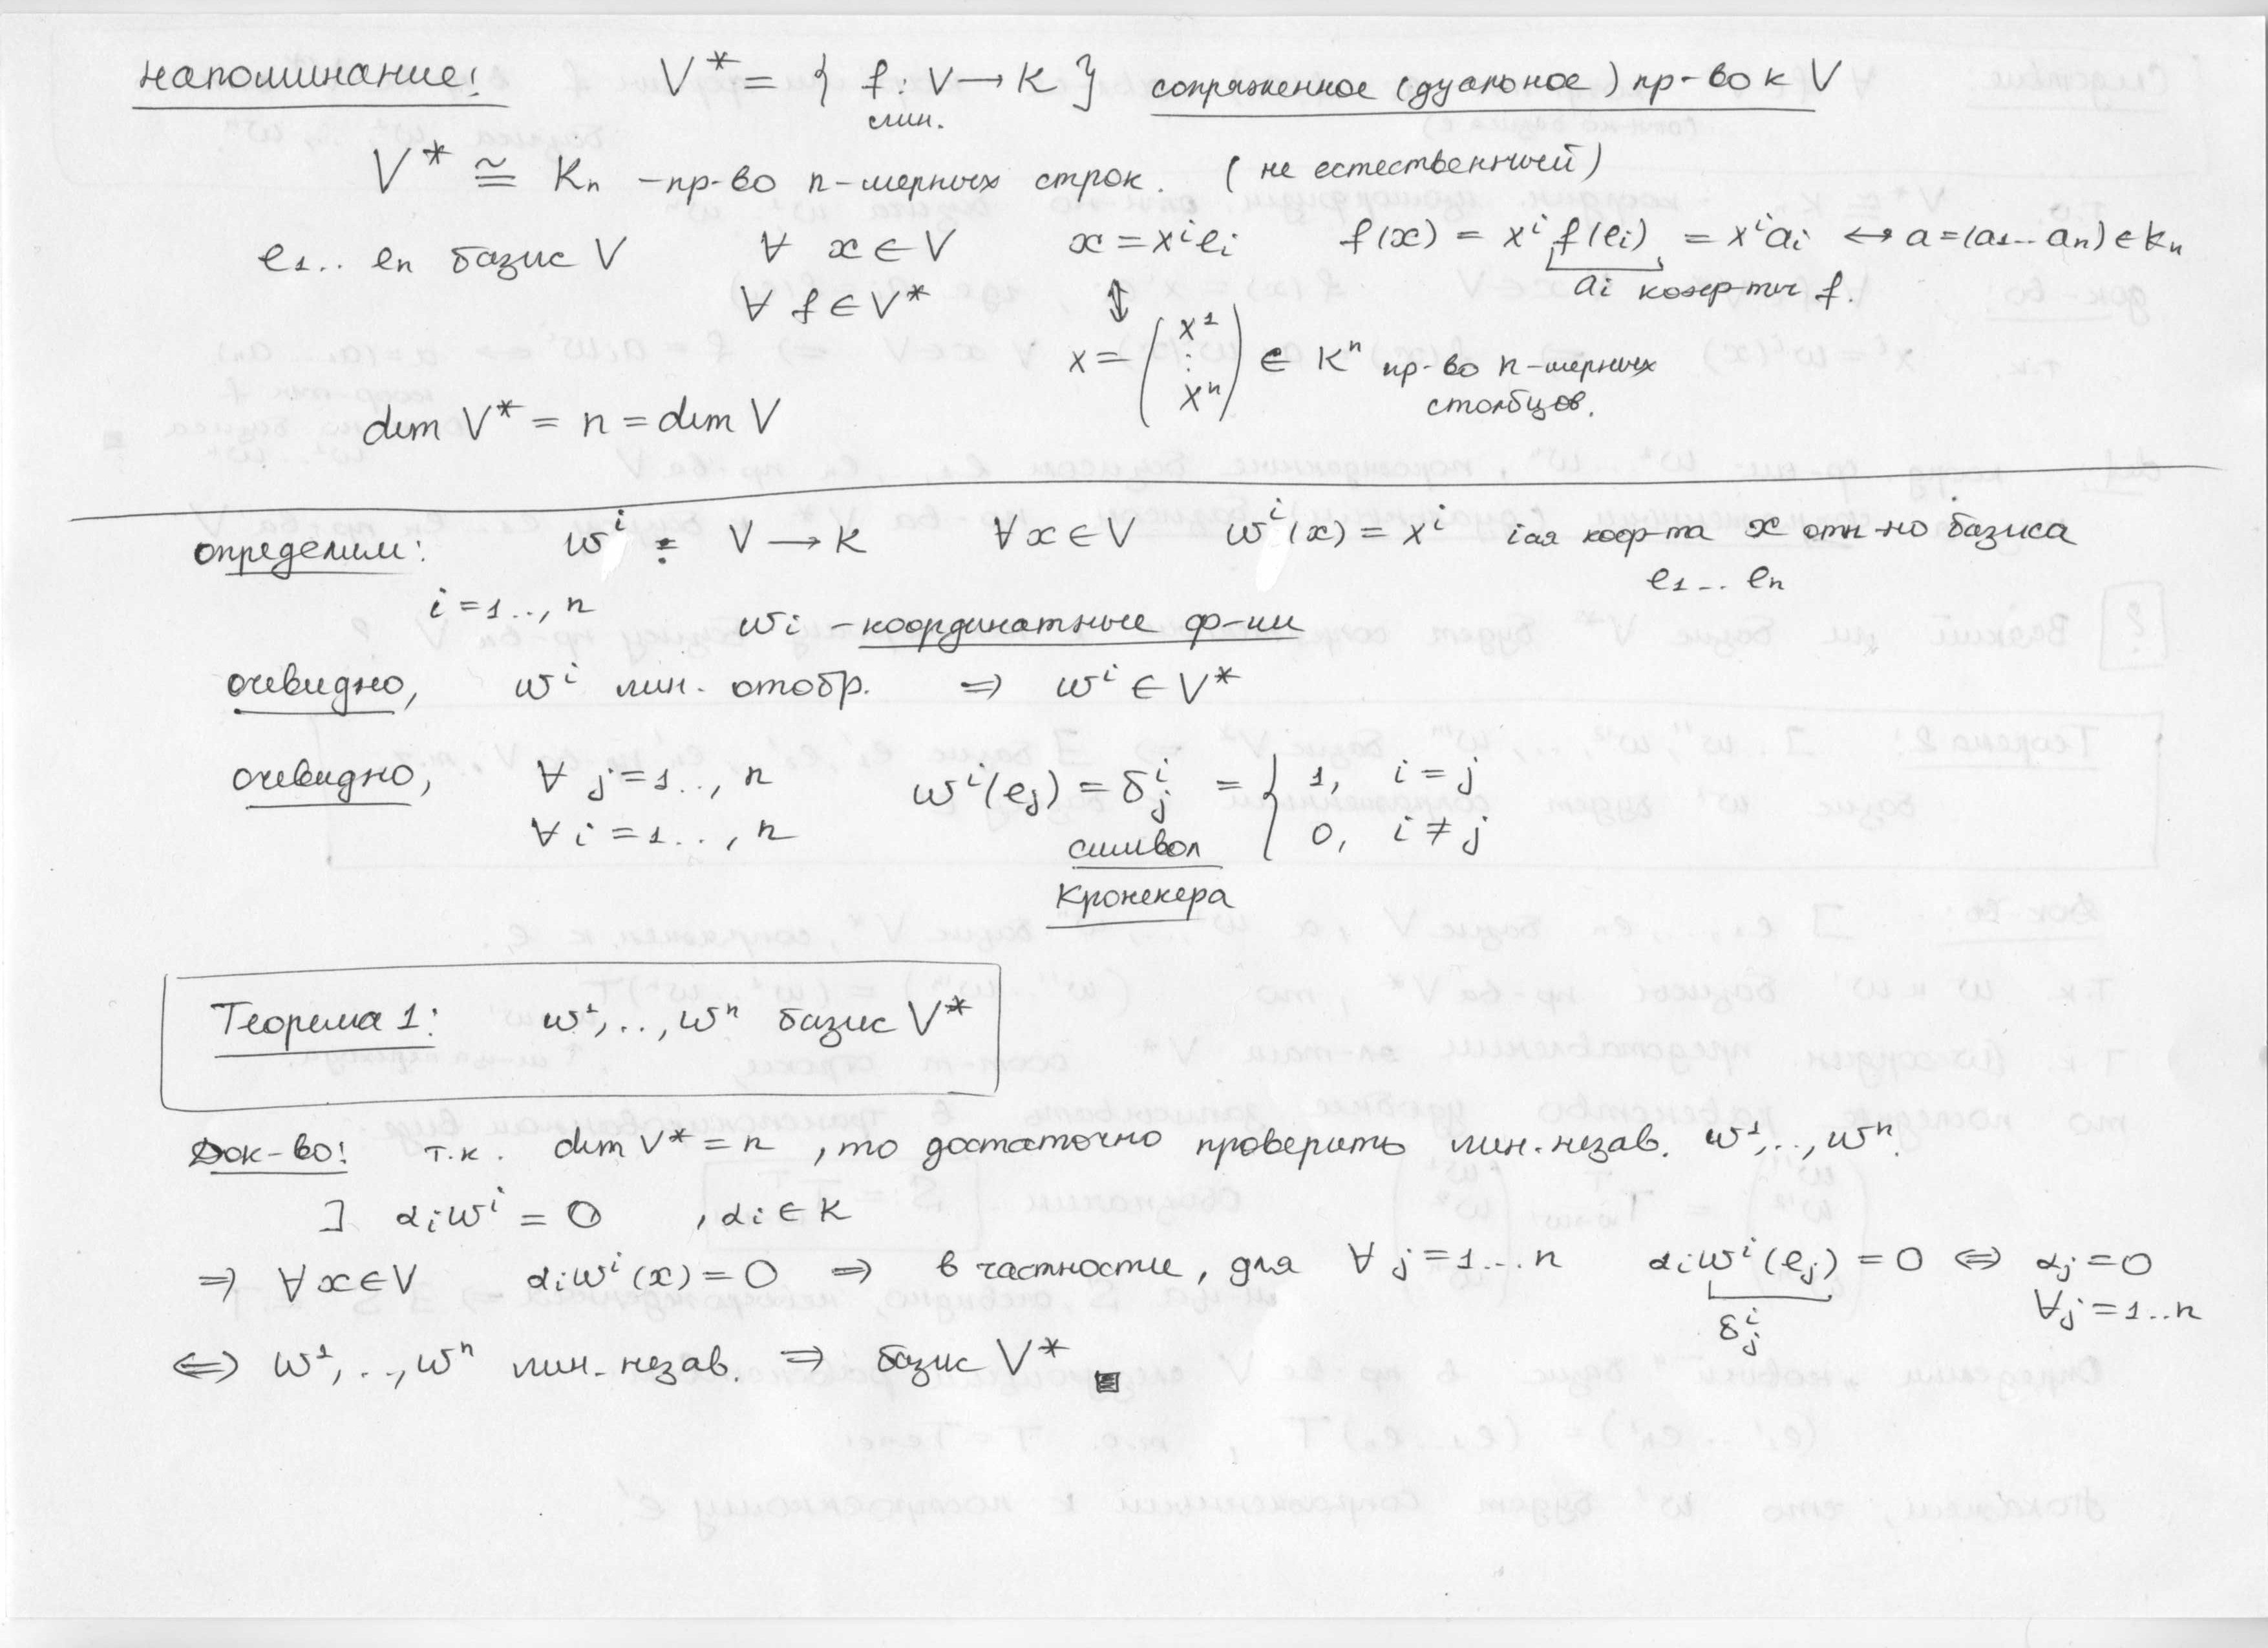
\includegraphics[height=0.49\textheight, width=\textwidth]{8_1-1}	
		\n
		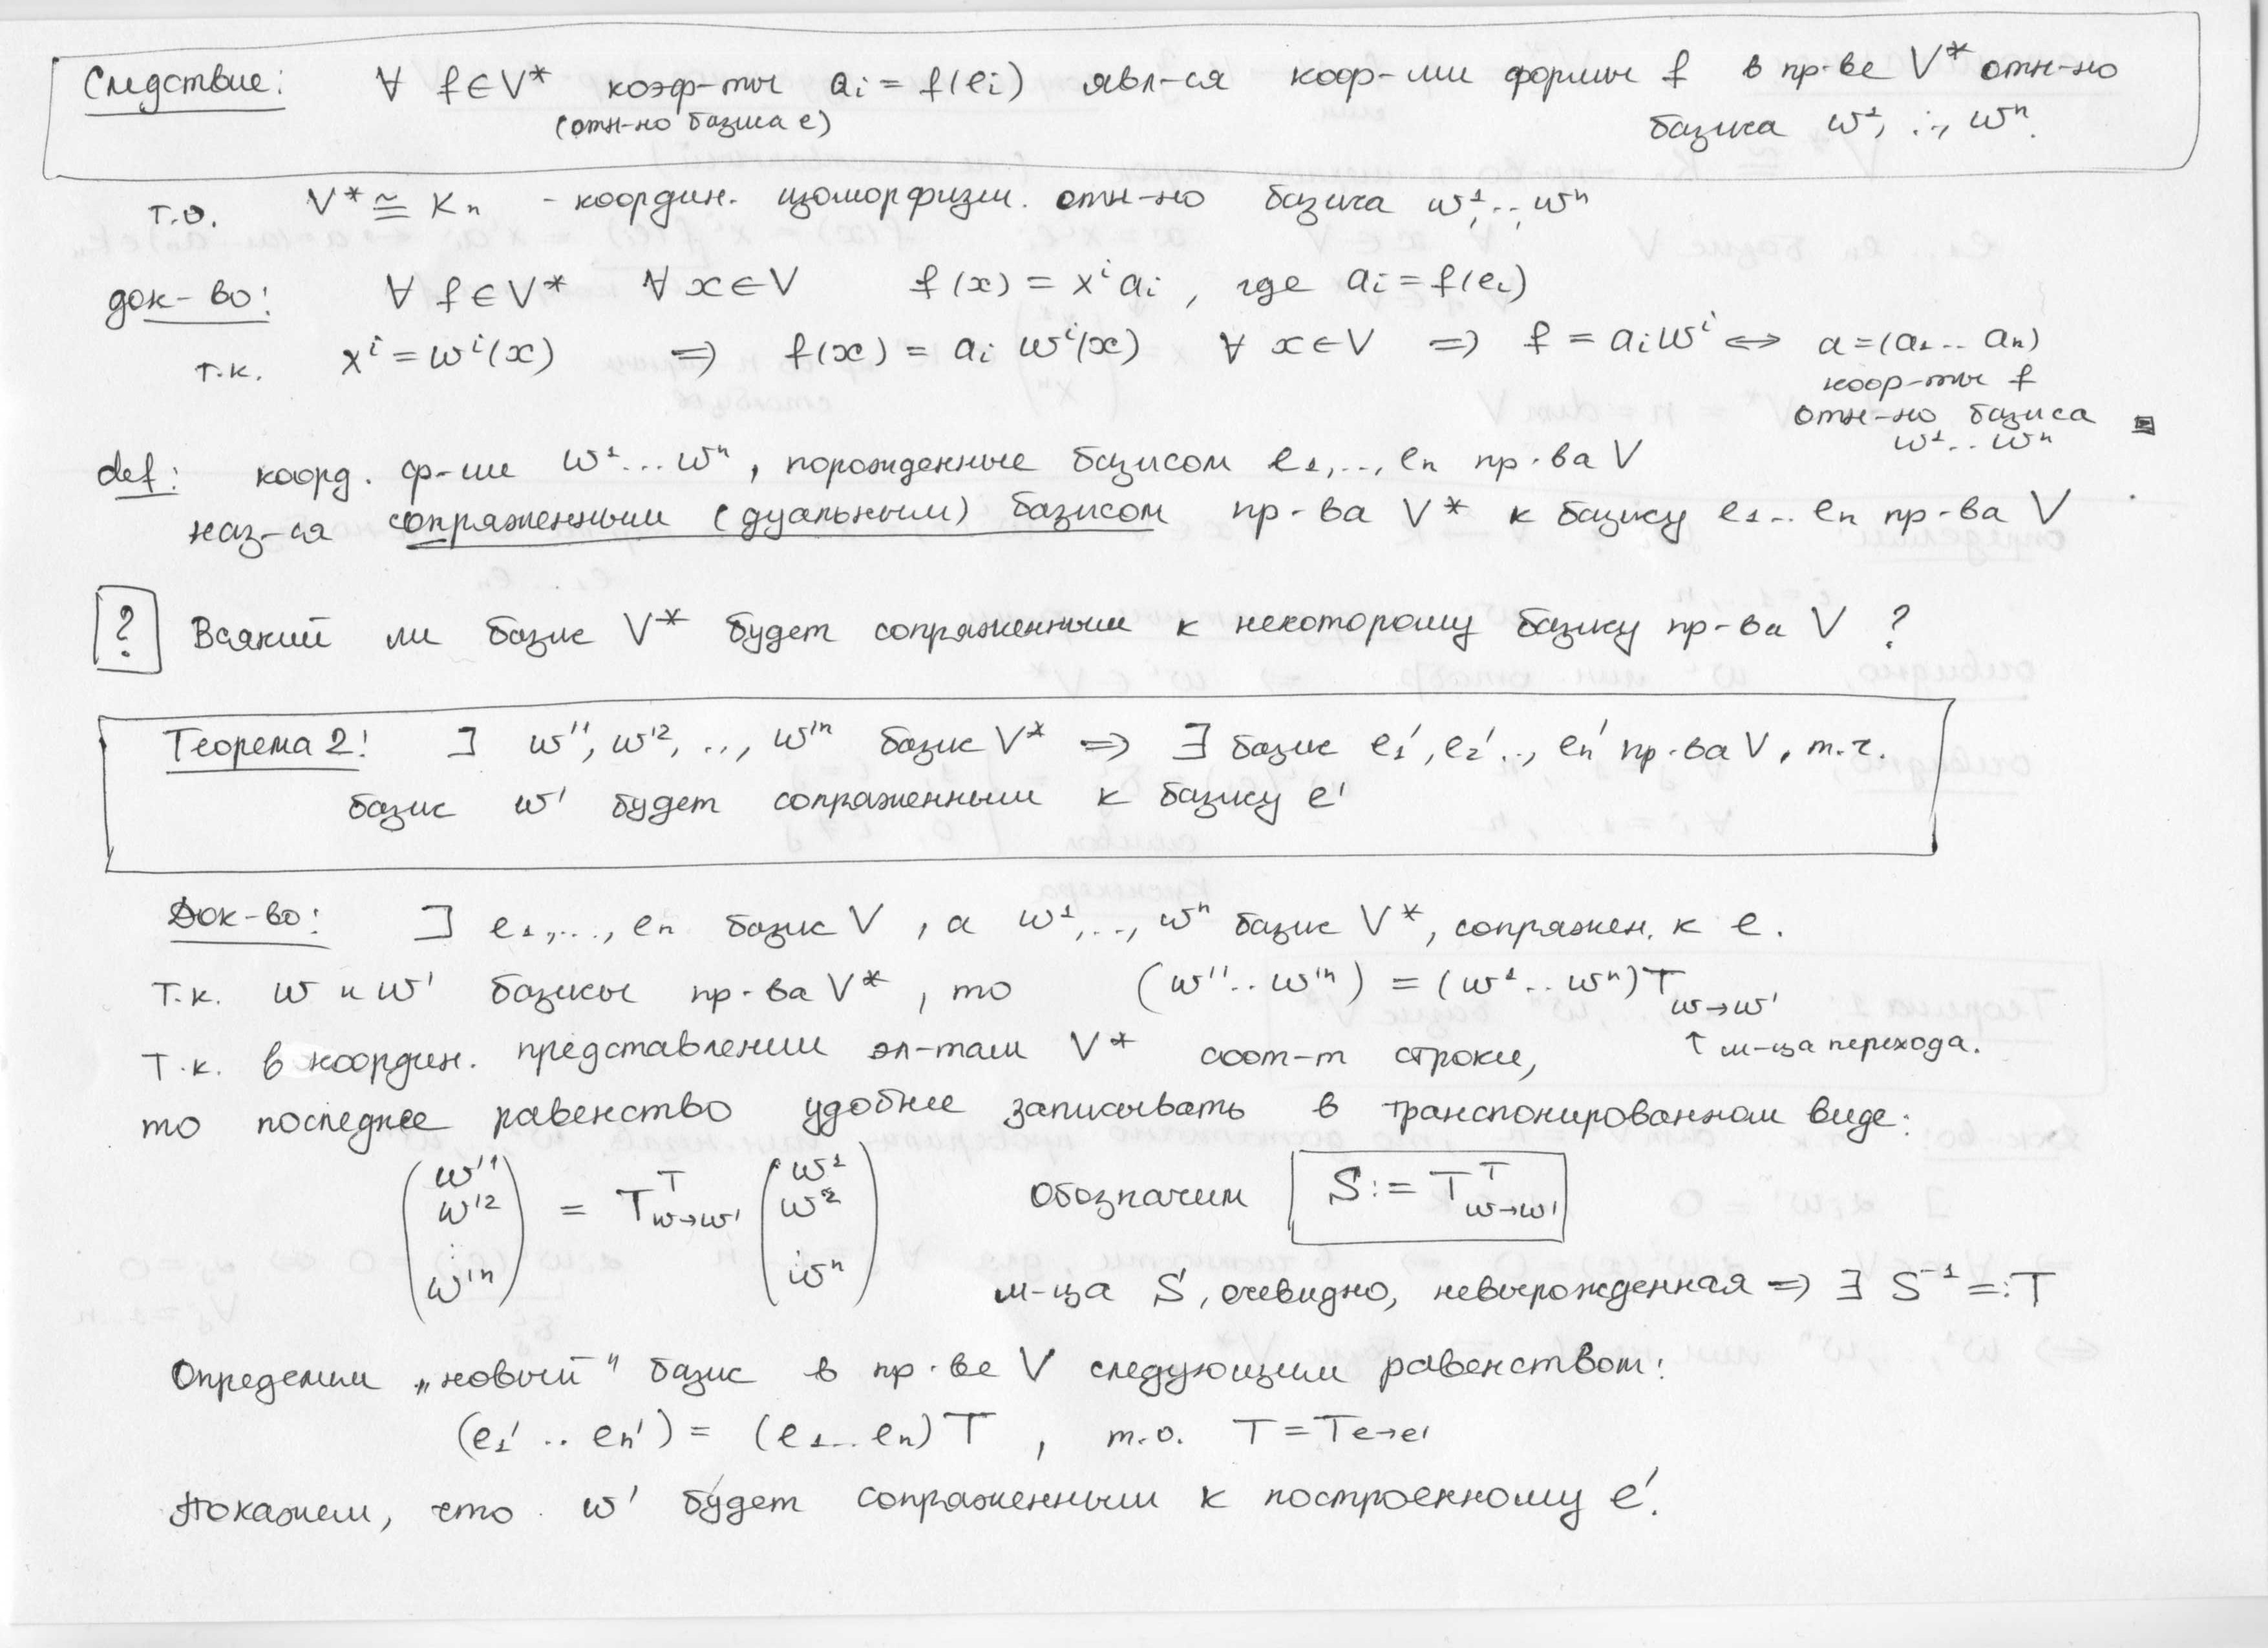
\includegraphics[height=0.49\textheight, width=\textwidth]{8_1-2}	
		\n
		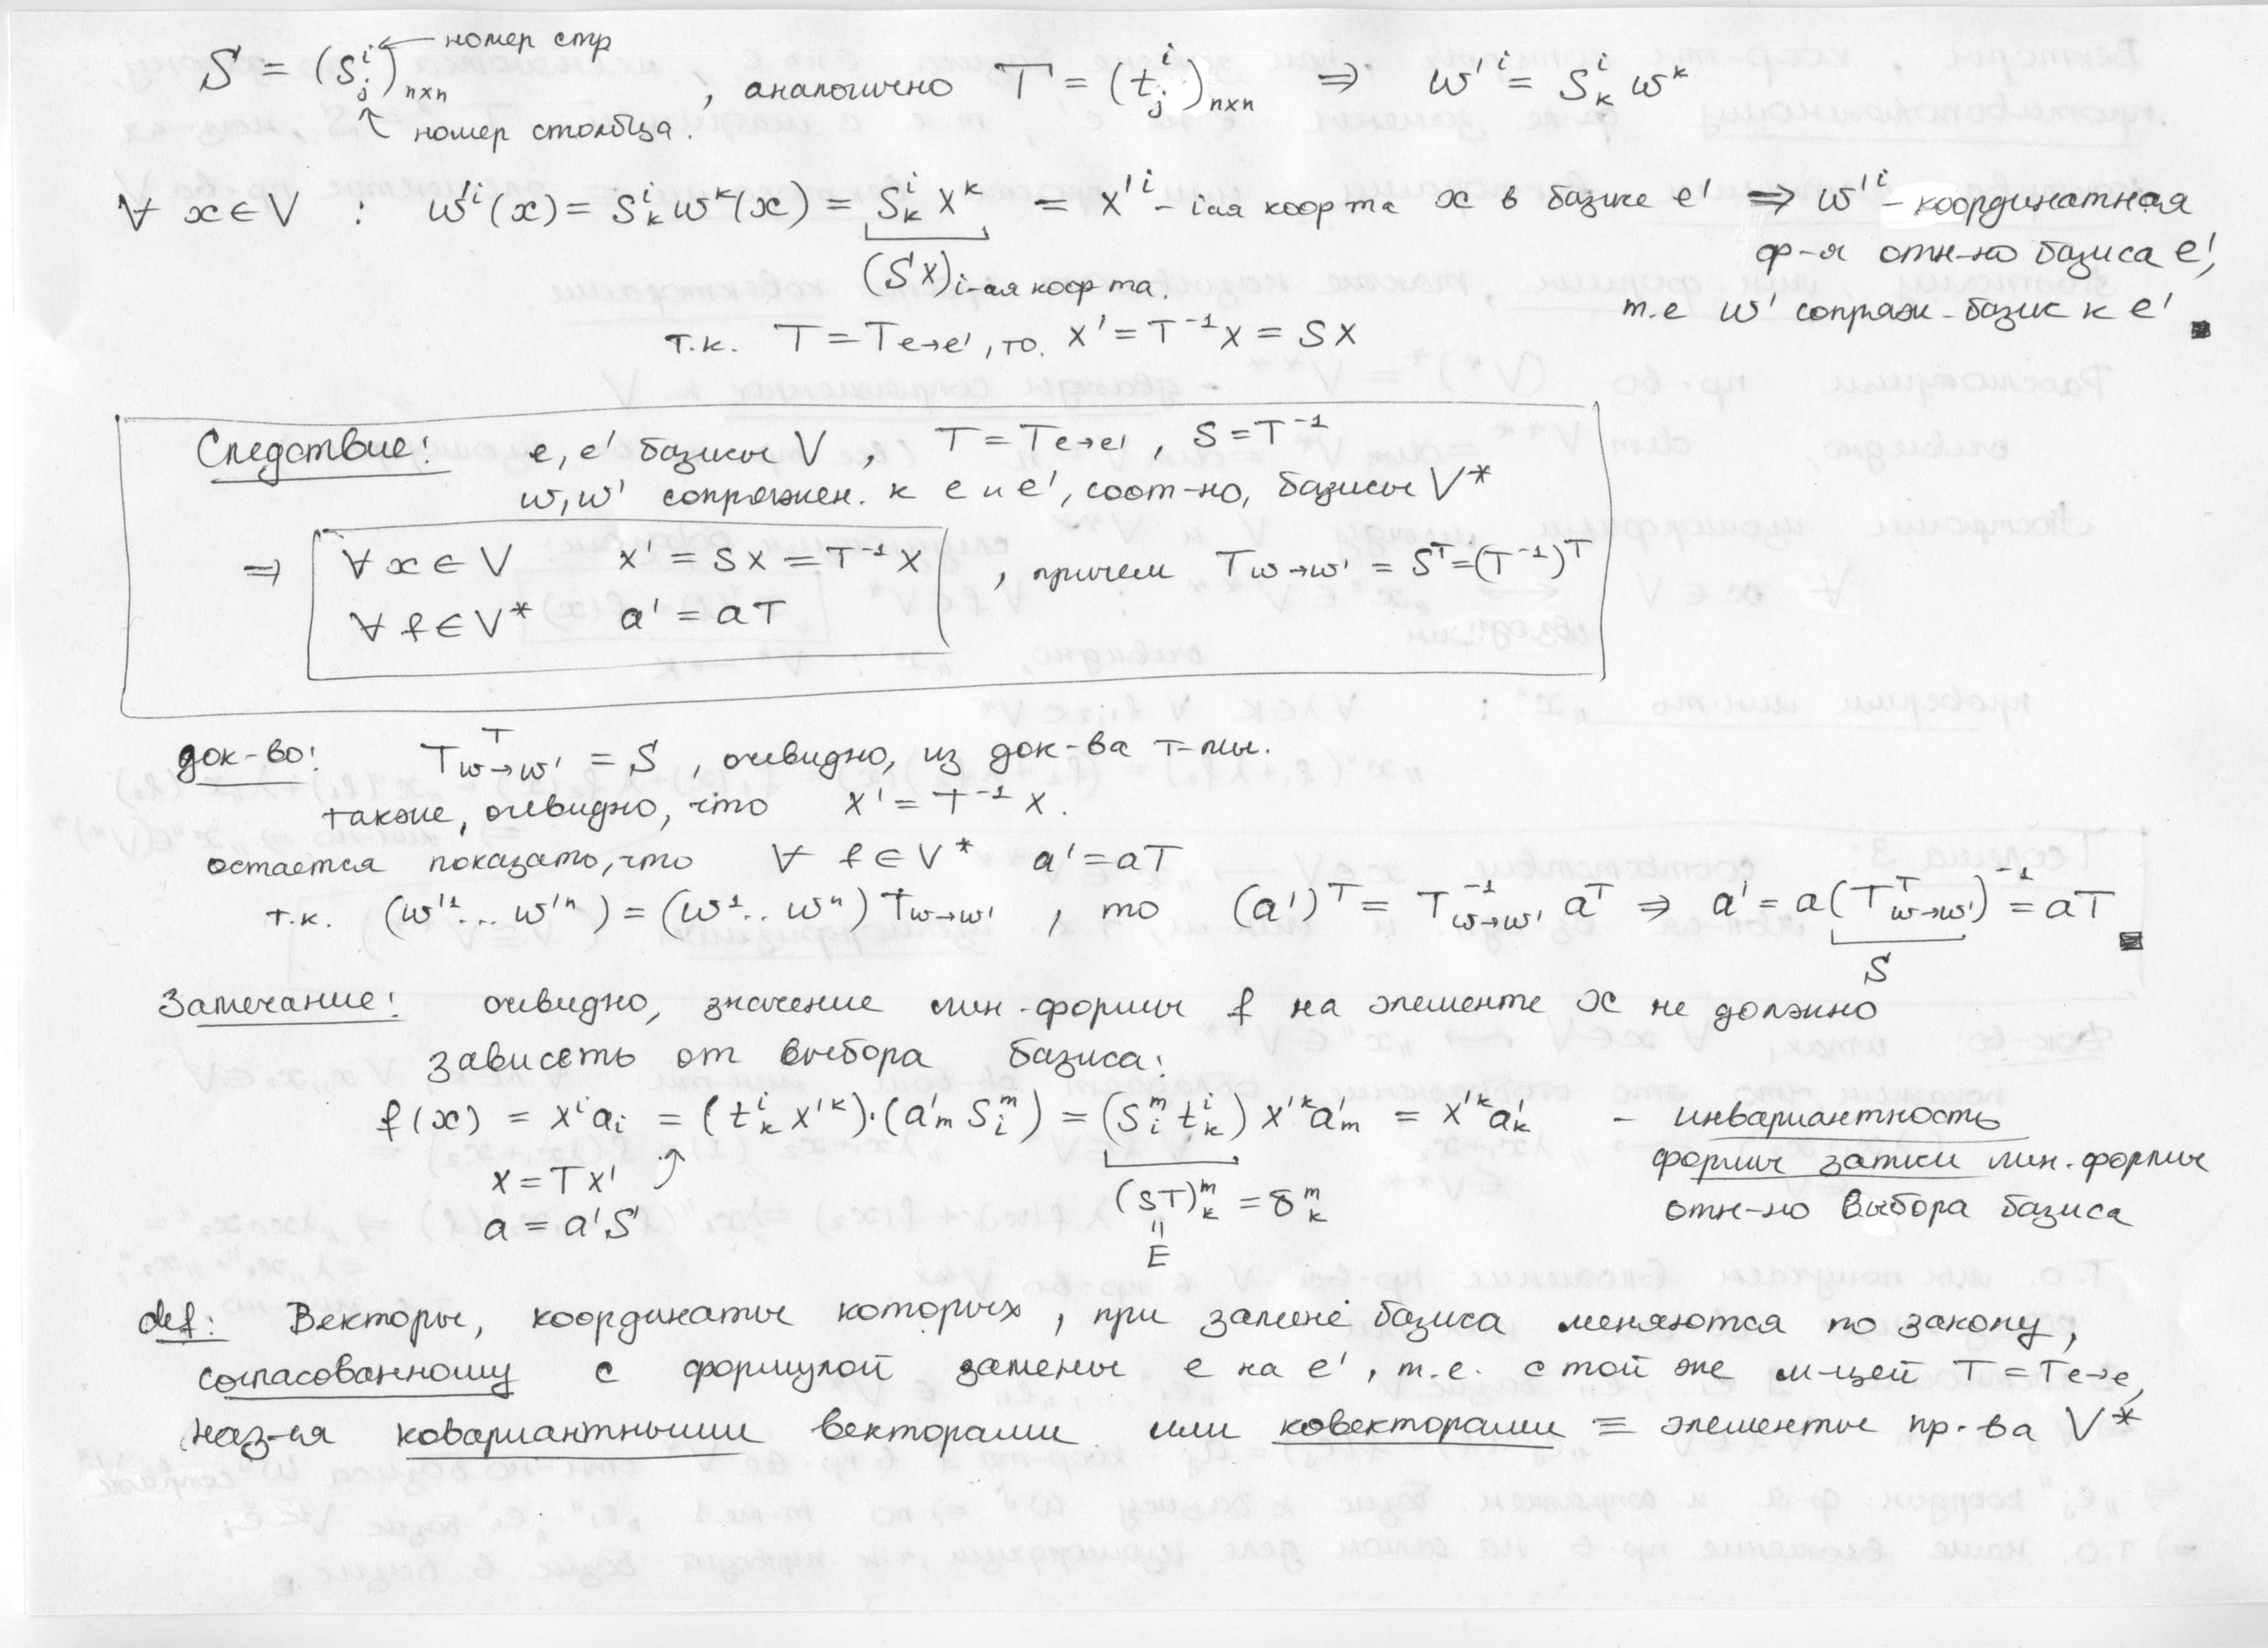
\includegraphics[height=0.49\textheight, width=\textwidth]{8_1-3}	
		\n
		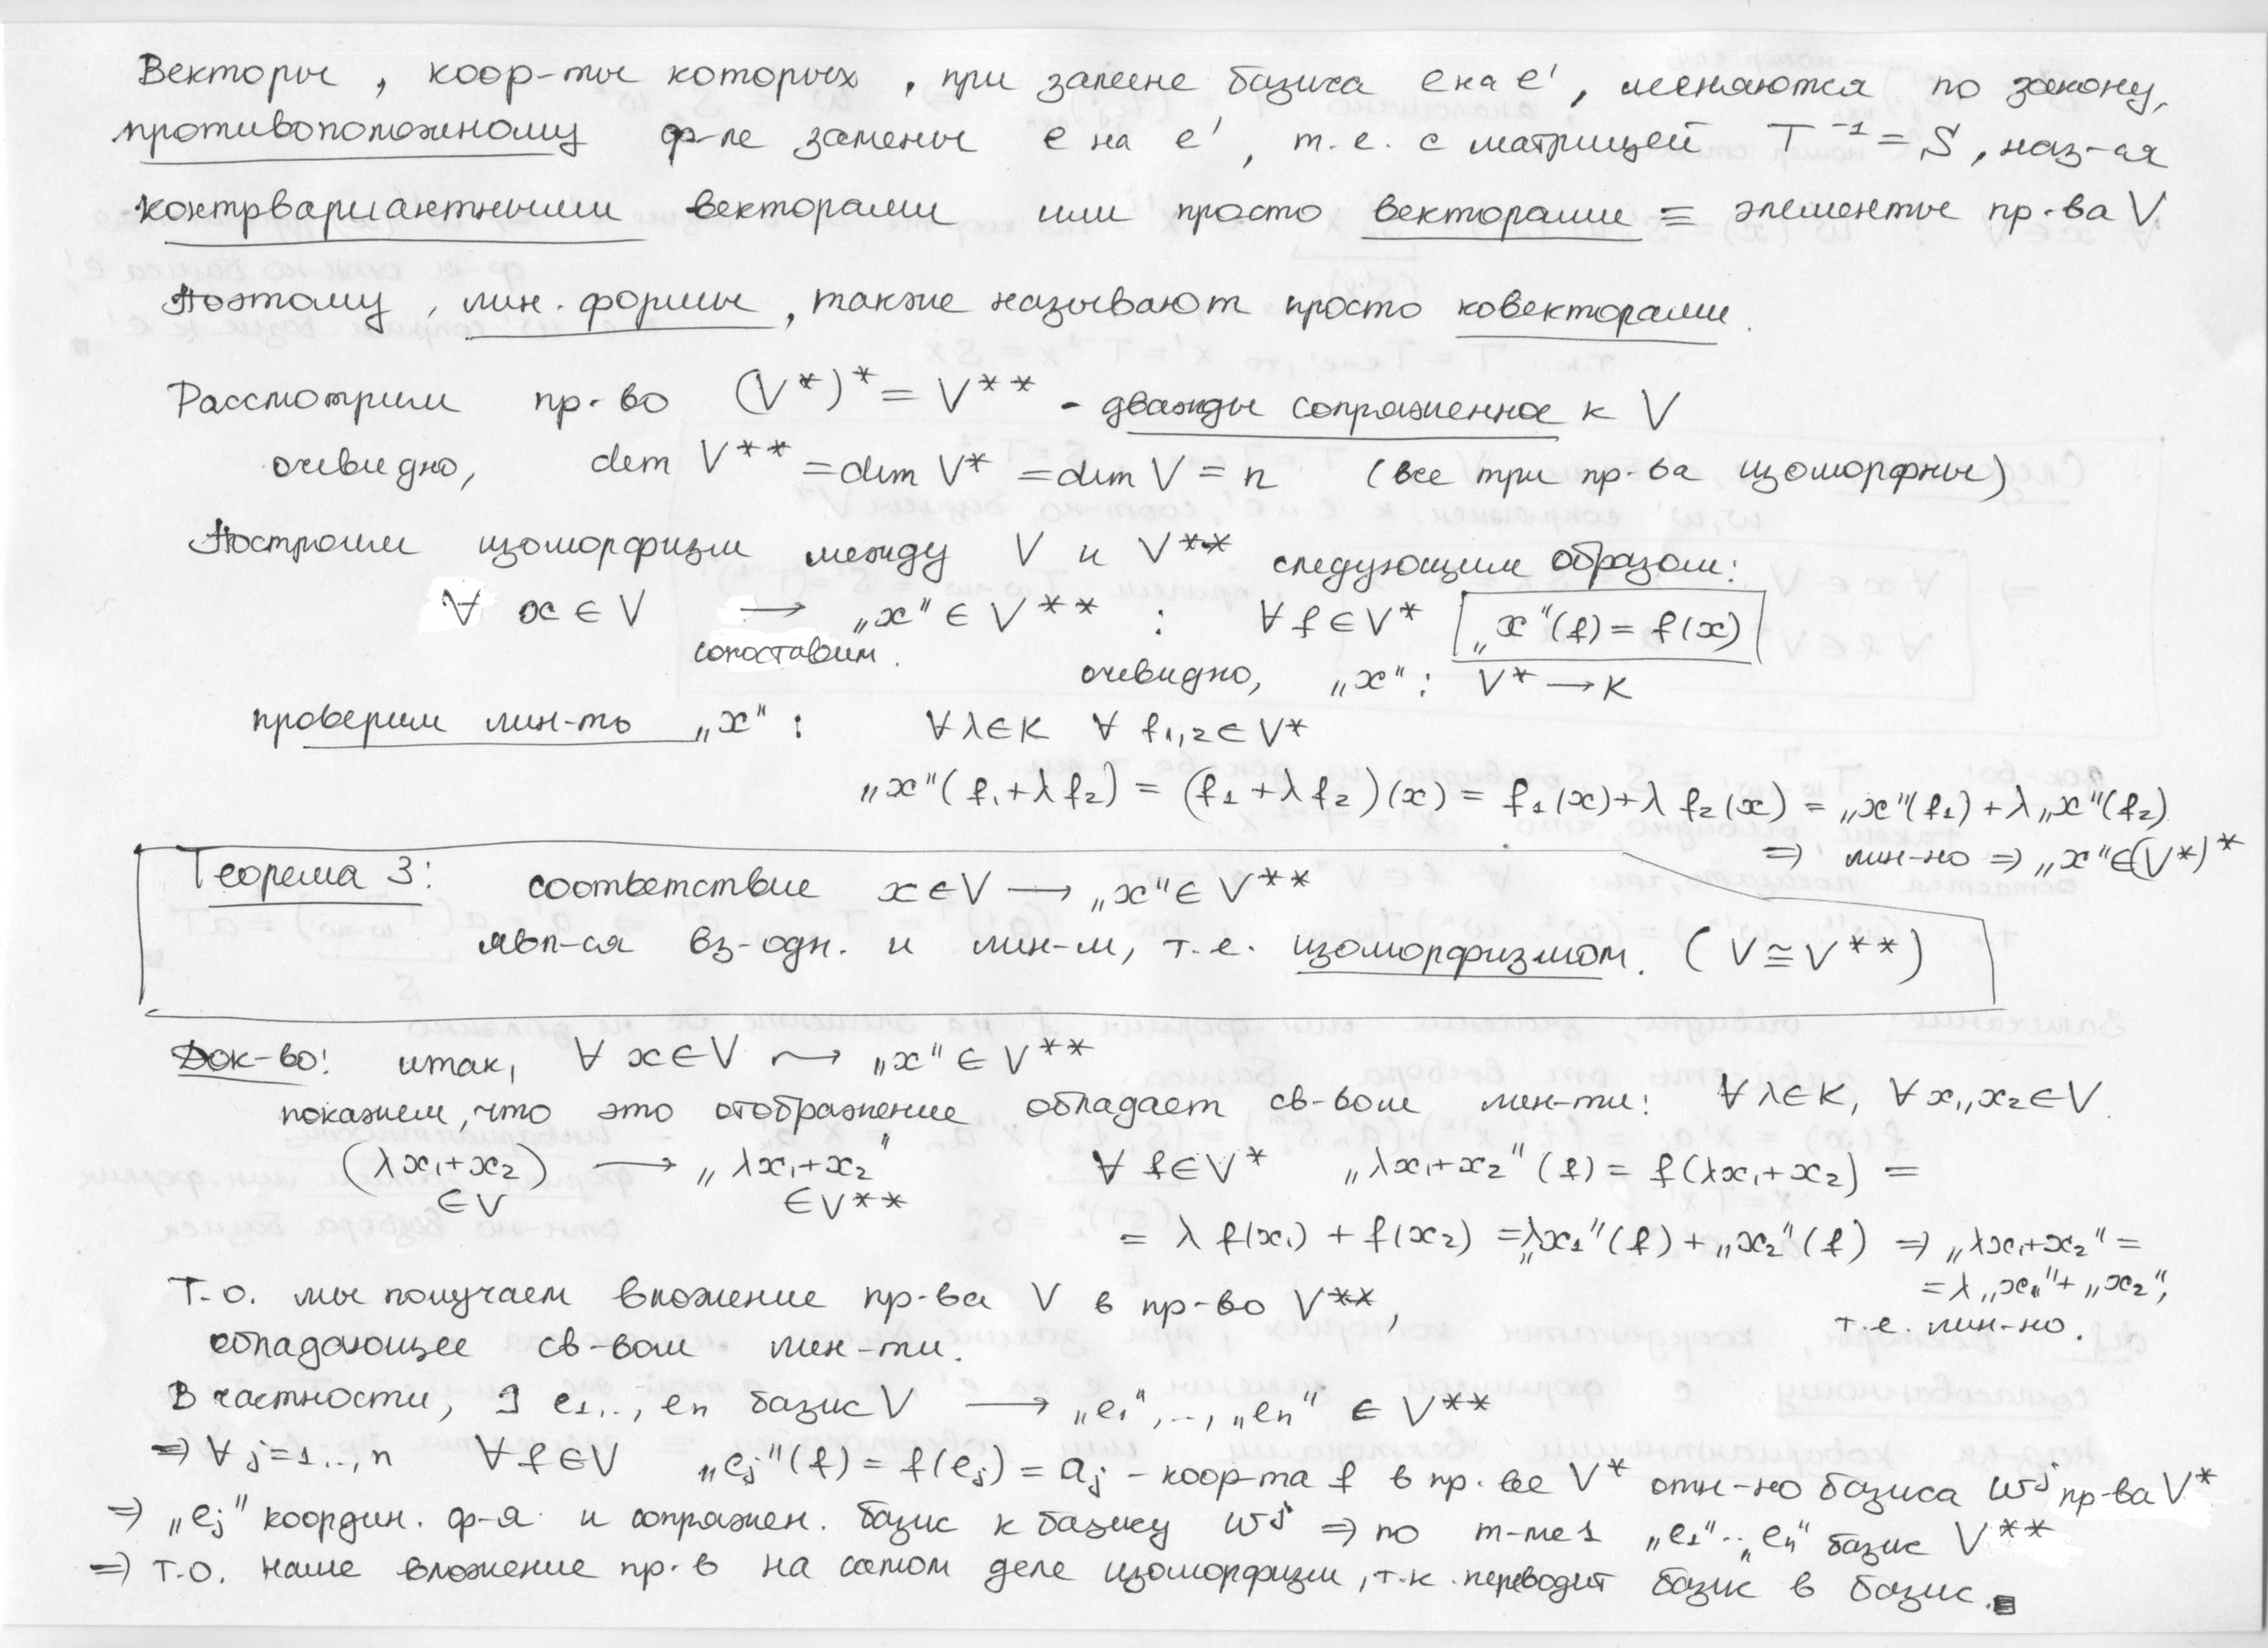
\includegraphics[height=0.49\textheight, width=\textwidth]{8_1-4}	
		\n
		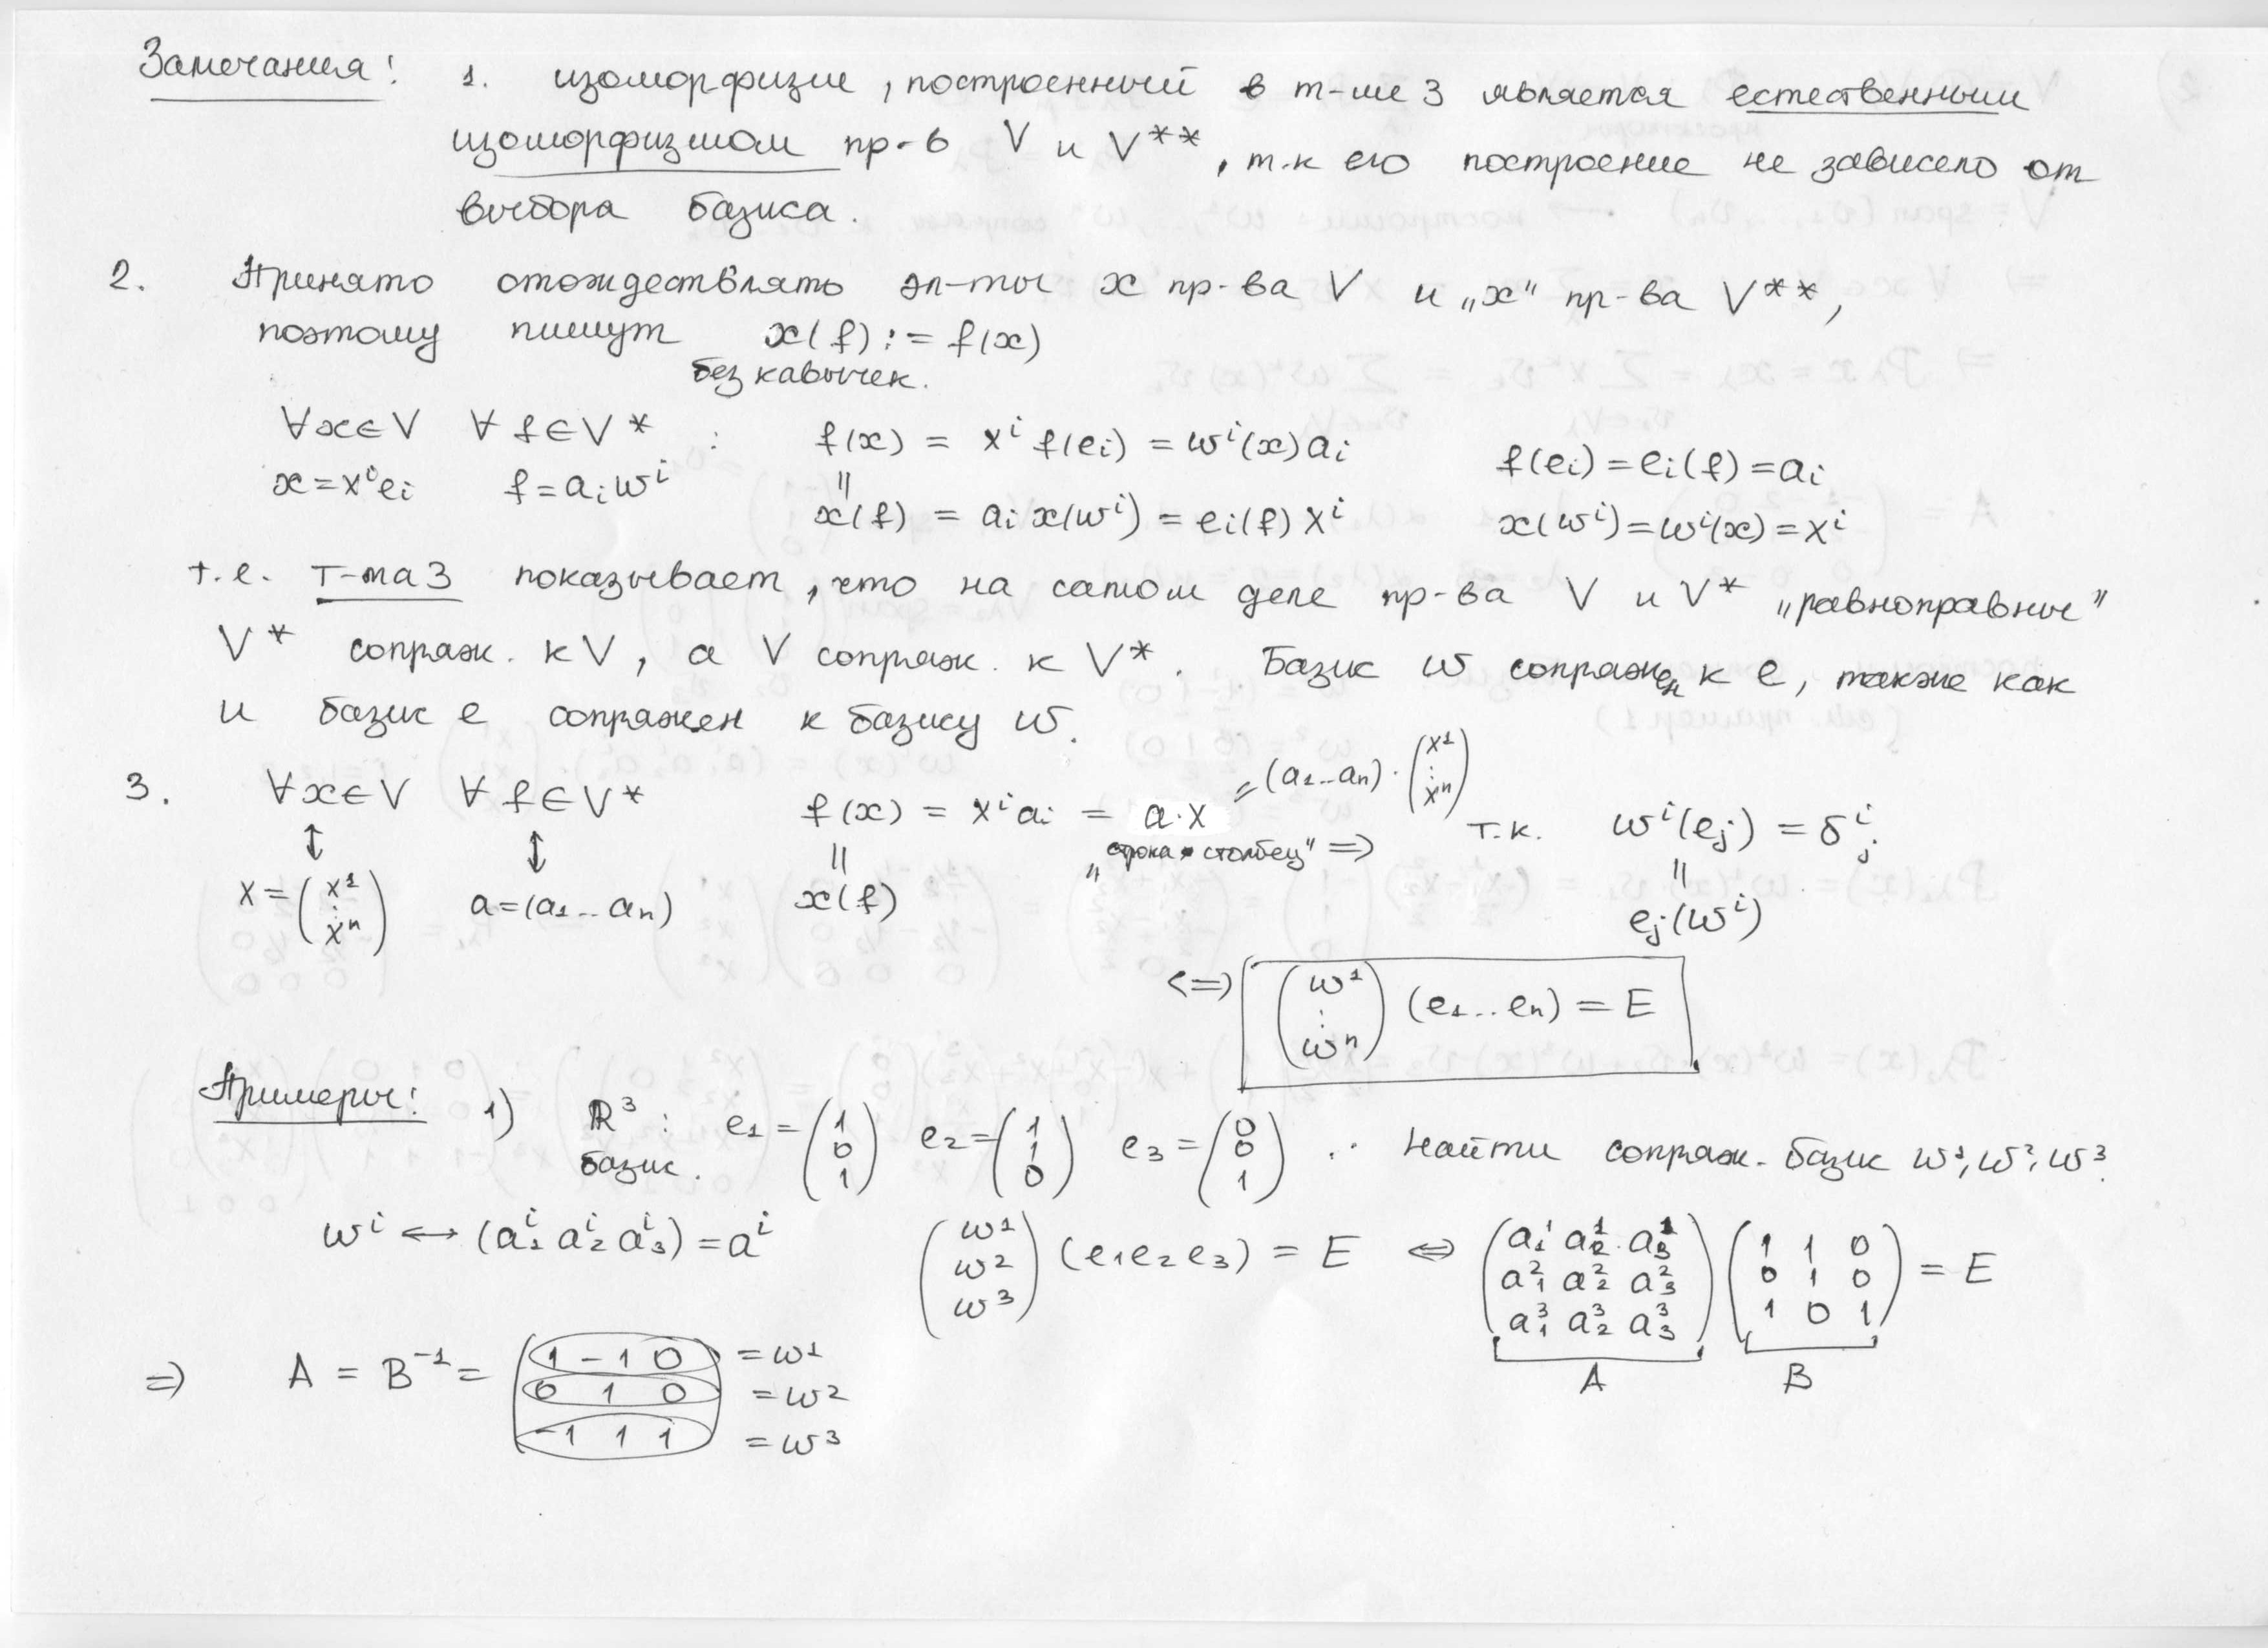
\includegraphics[height=0.49\textheight, width=\textwidth]{8_1-5}	
		\n
		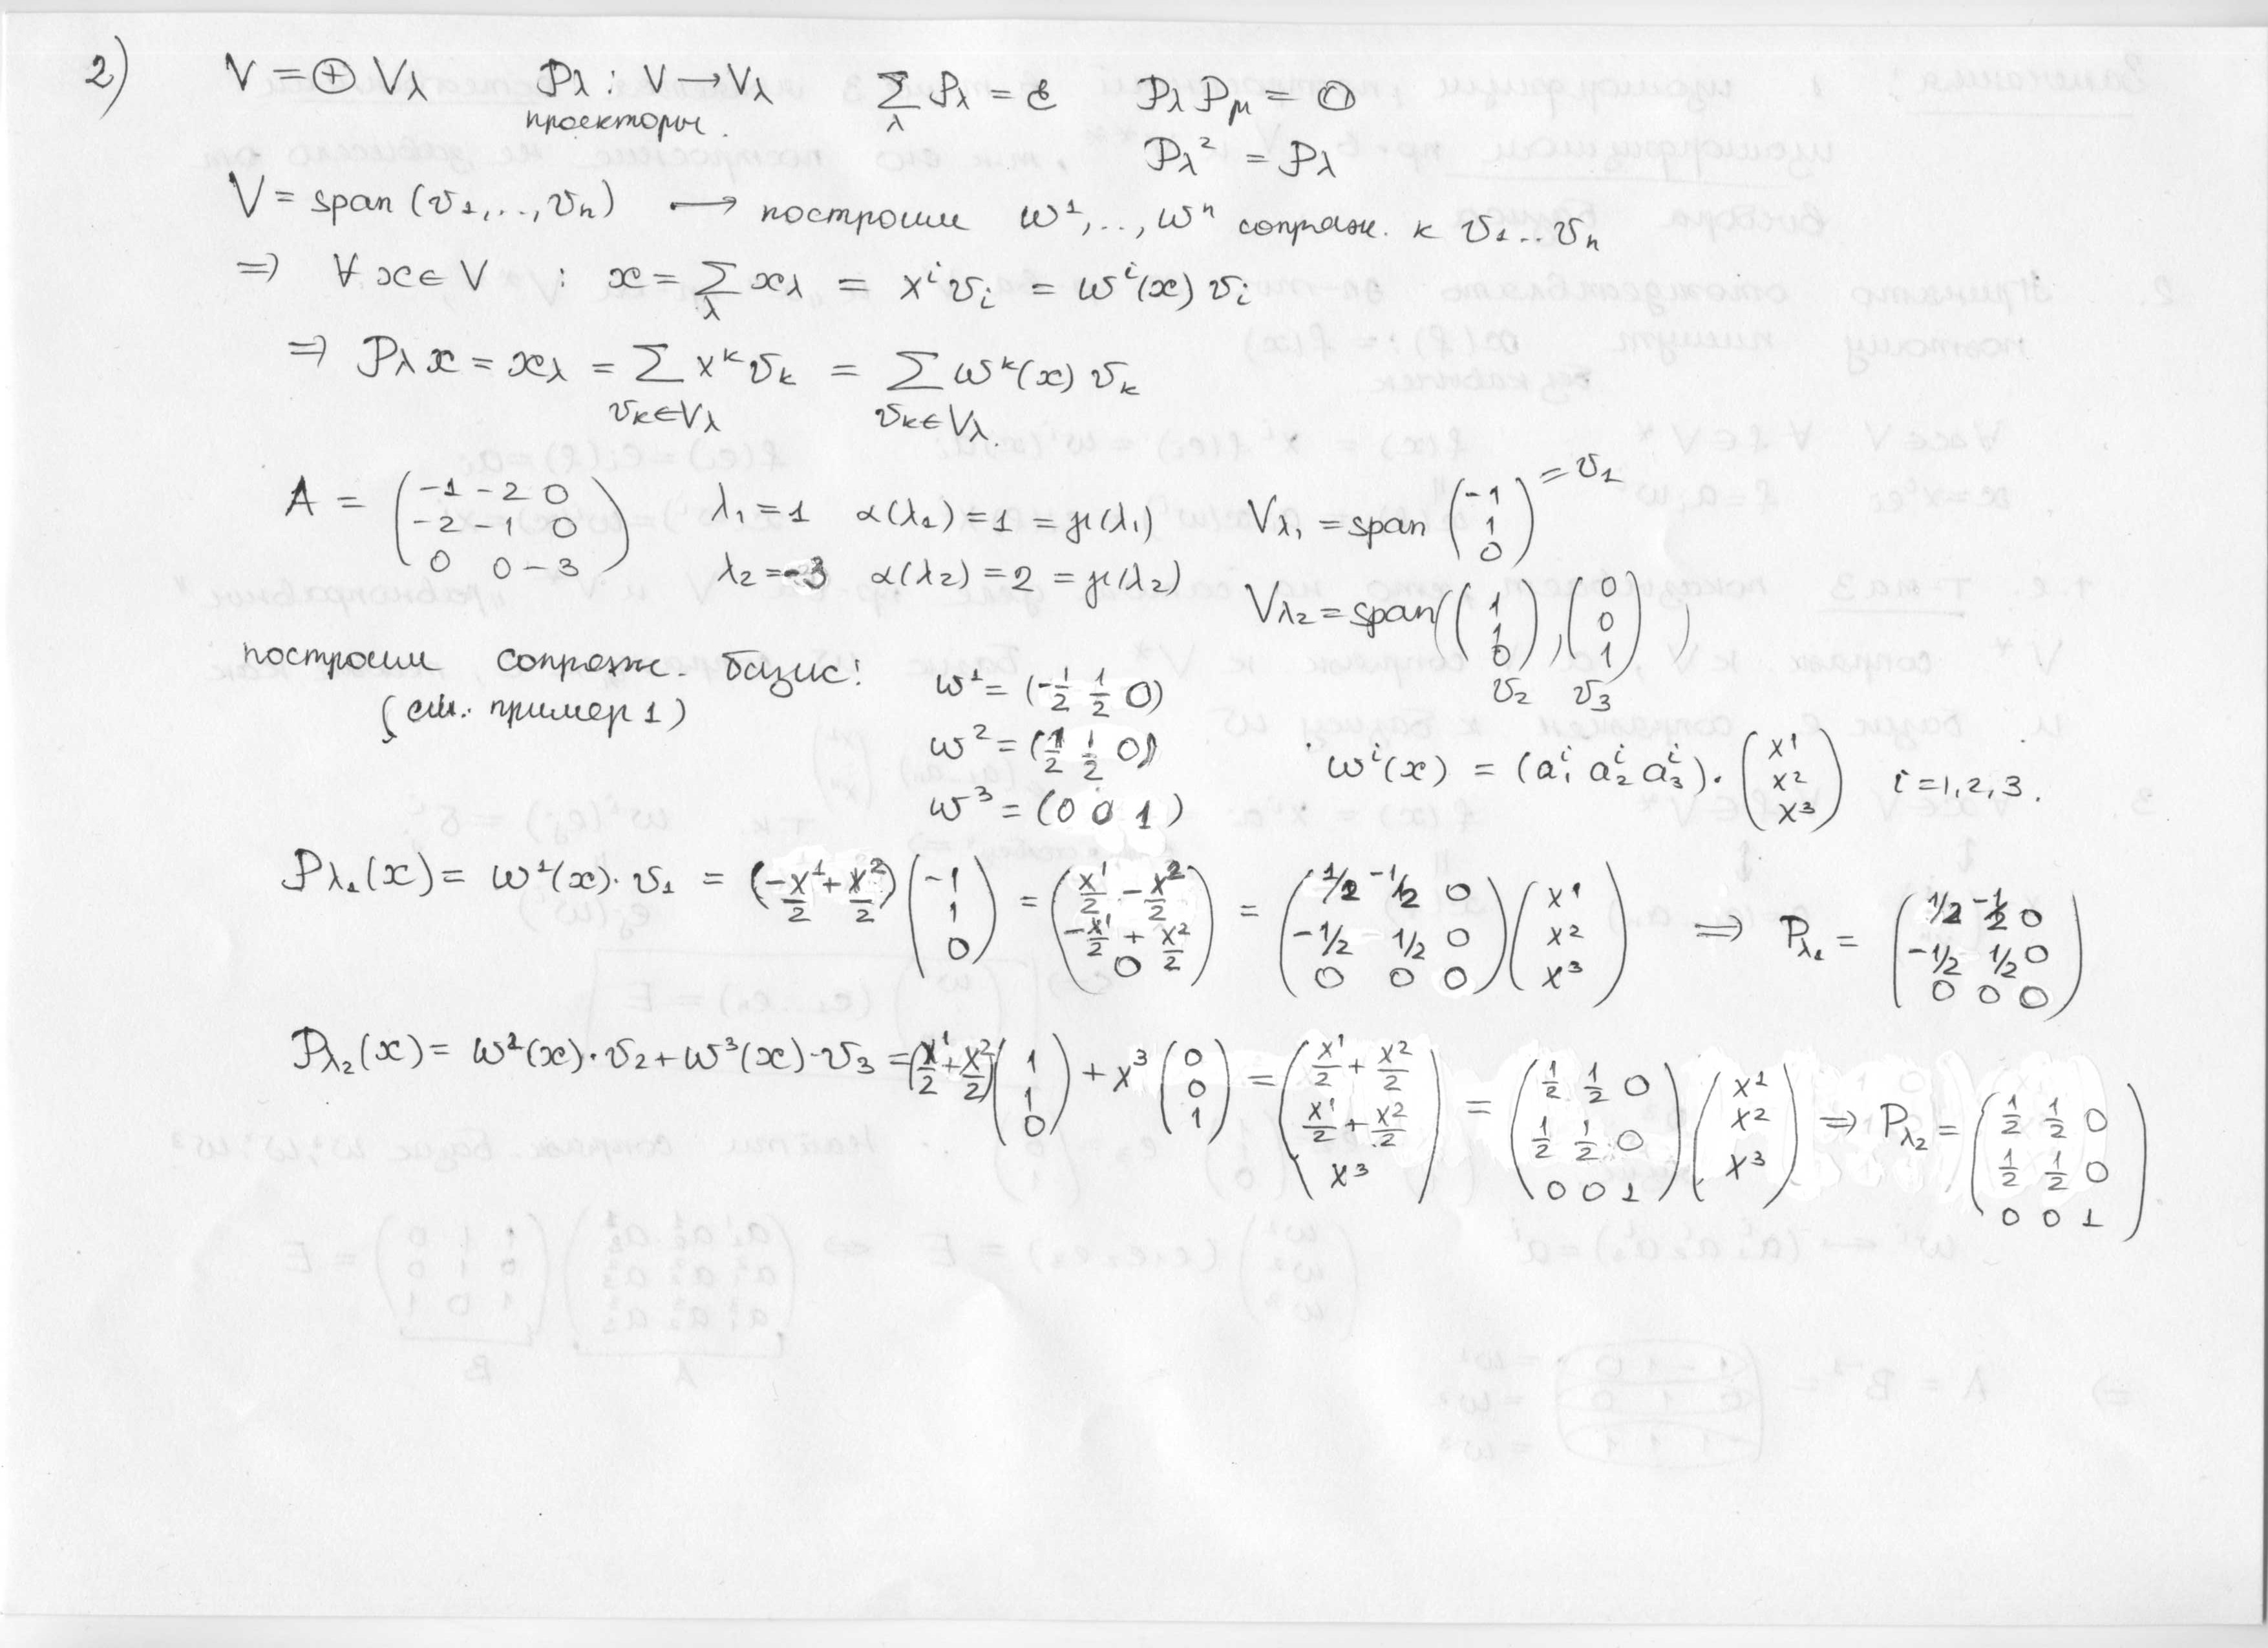
\includegraphics[height=0.49\textheight, width=\textwidth]{8_1-6}	
		\n
	\subsection{Два определения тензора. Многомерная матрица. Линейной пространство тензоров.}
	 		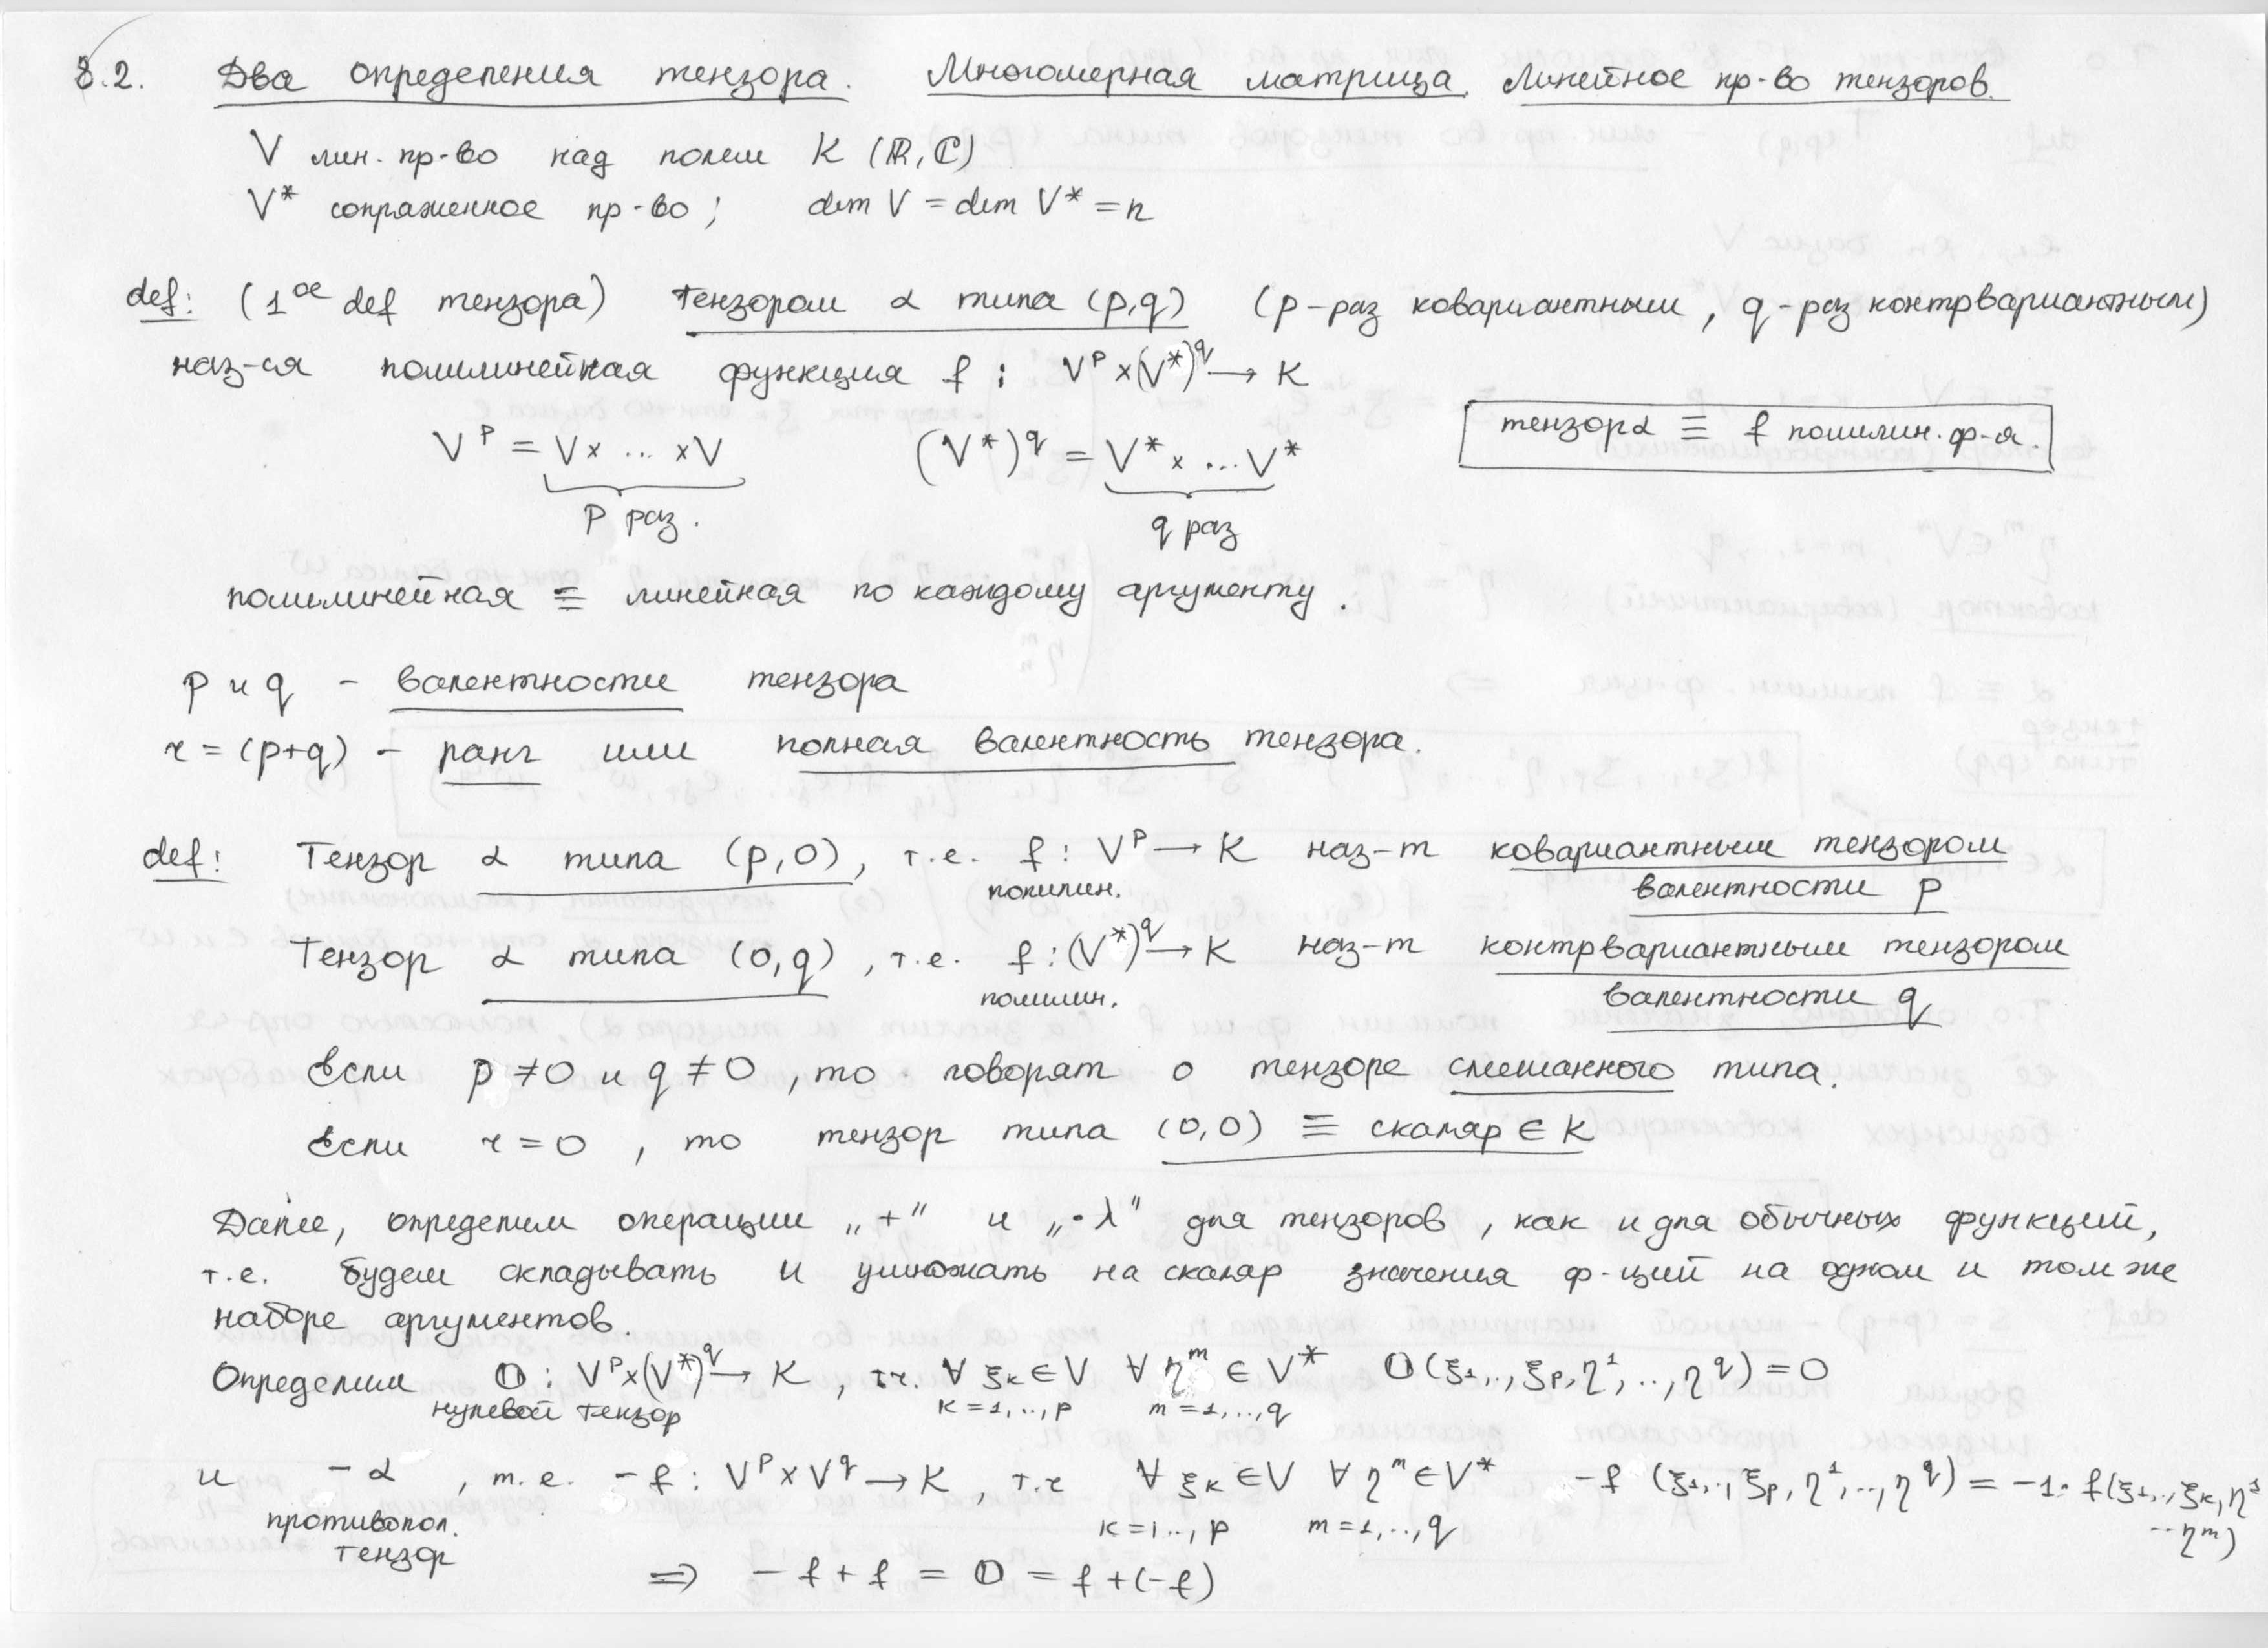
\includegraphics[height=0.49\textheight, width=\textwidth]{8_2-1}	
		\n
		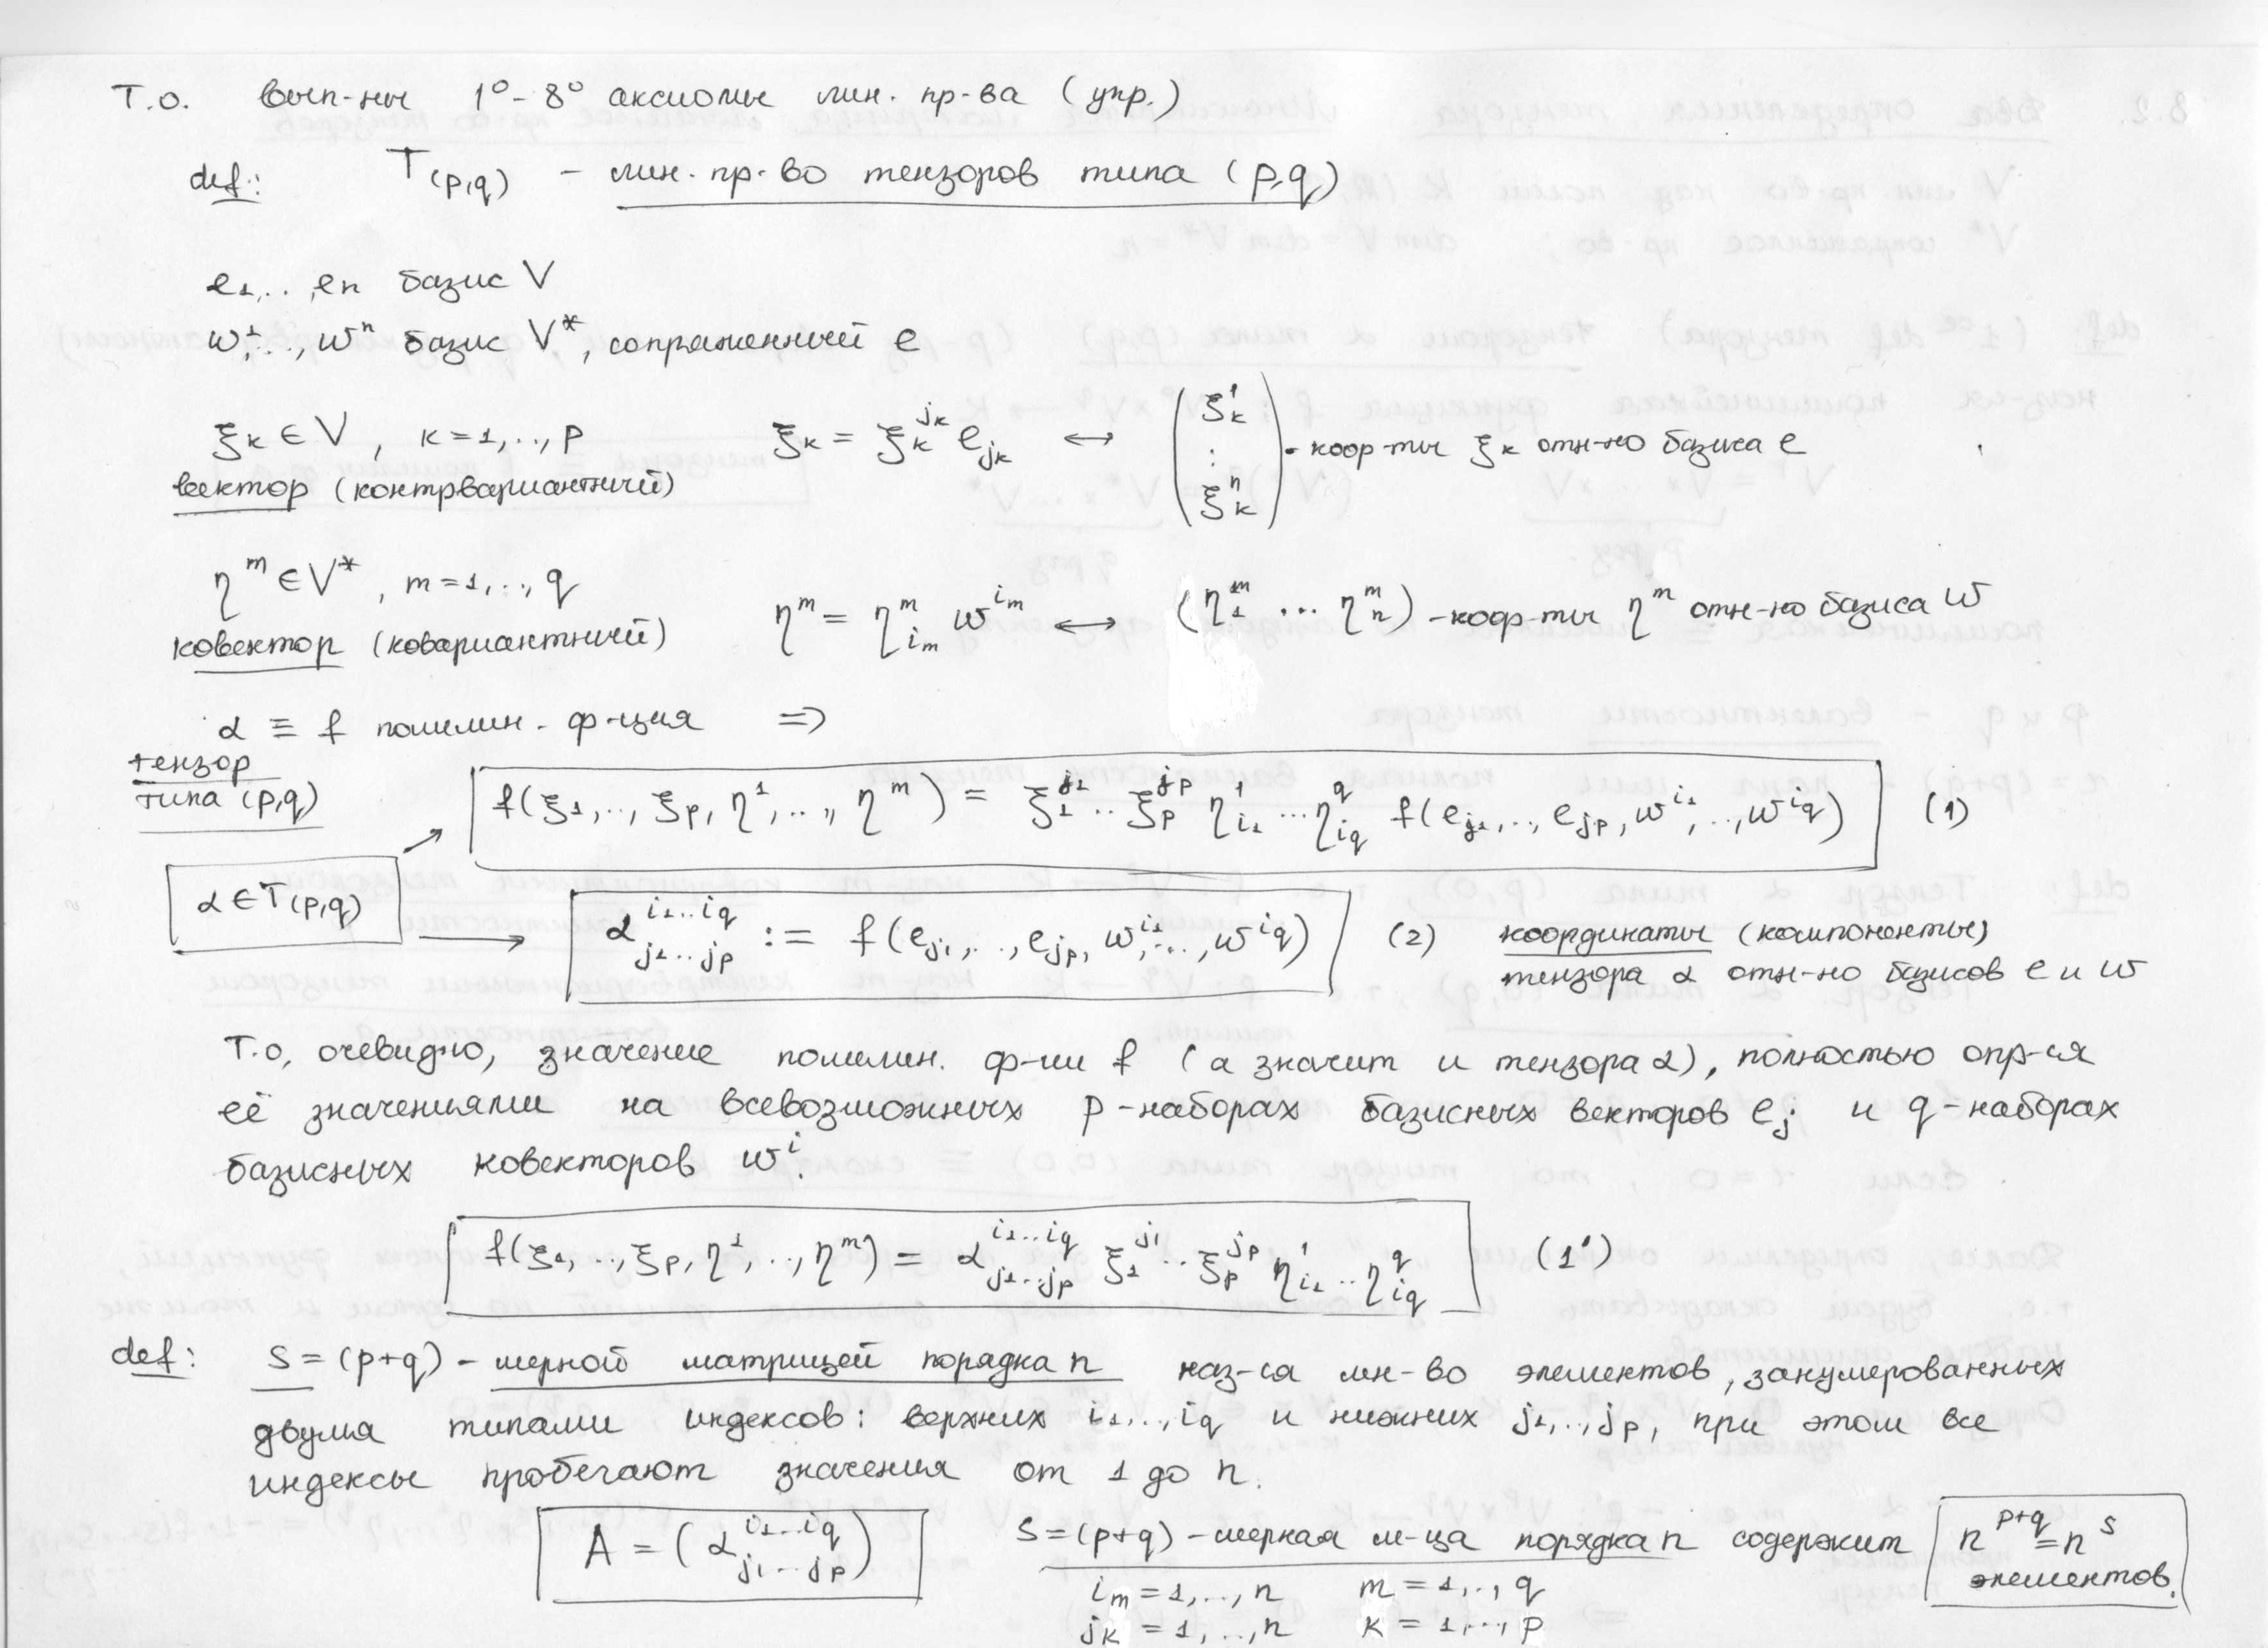
\includegraphics[height=0.49\textheight, width=\textwidth]{8_2-2}	
		\n
		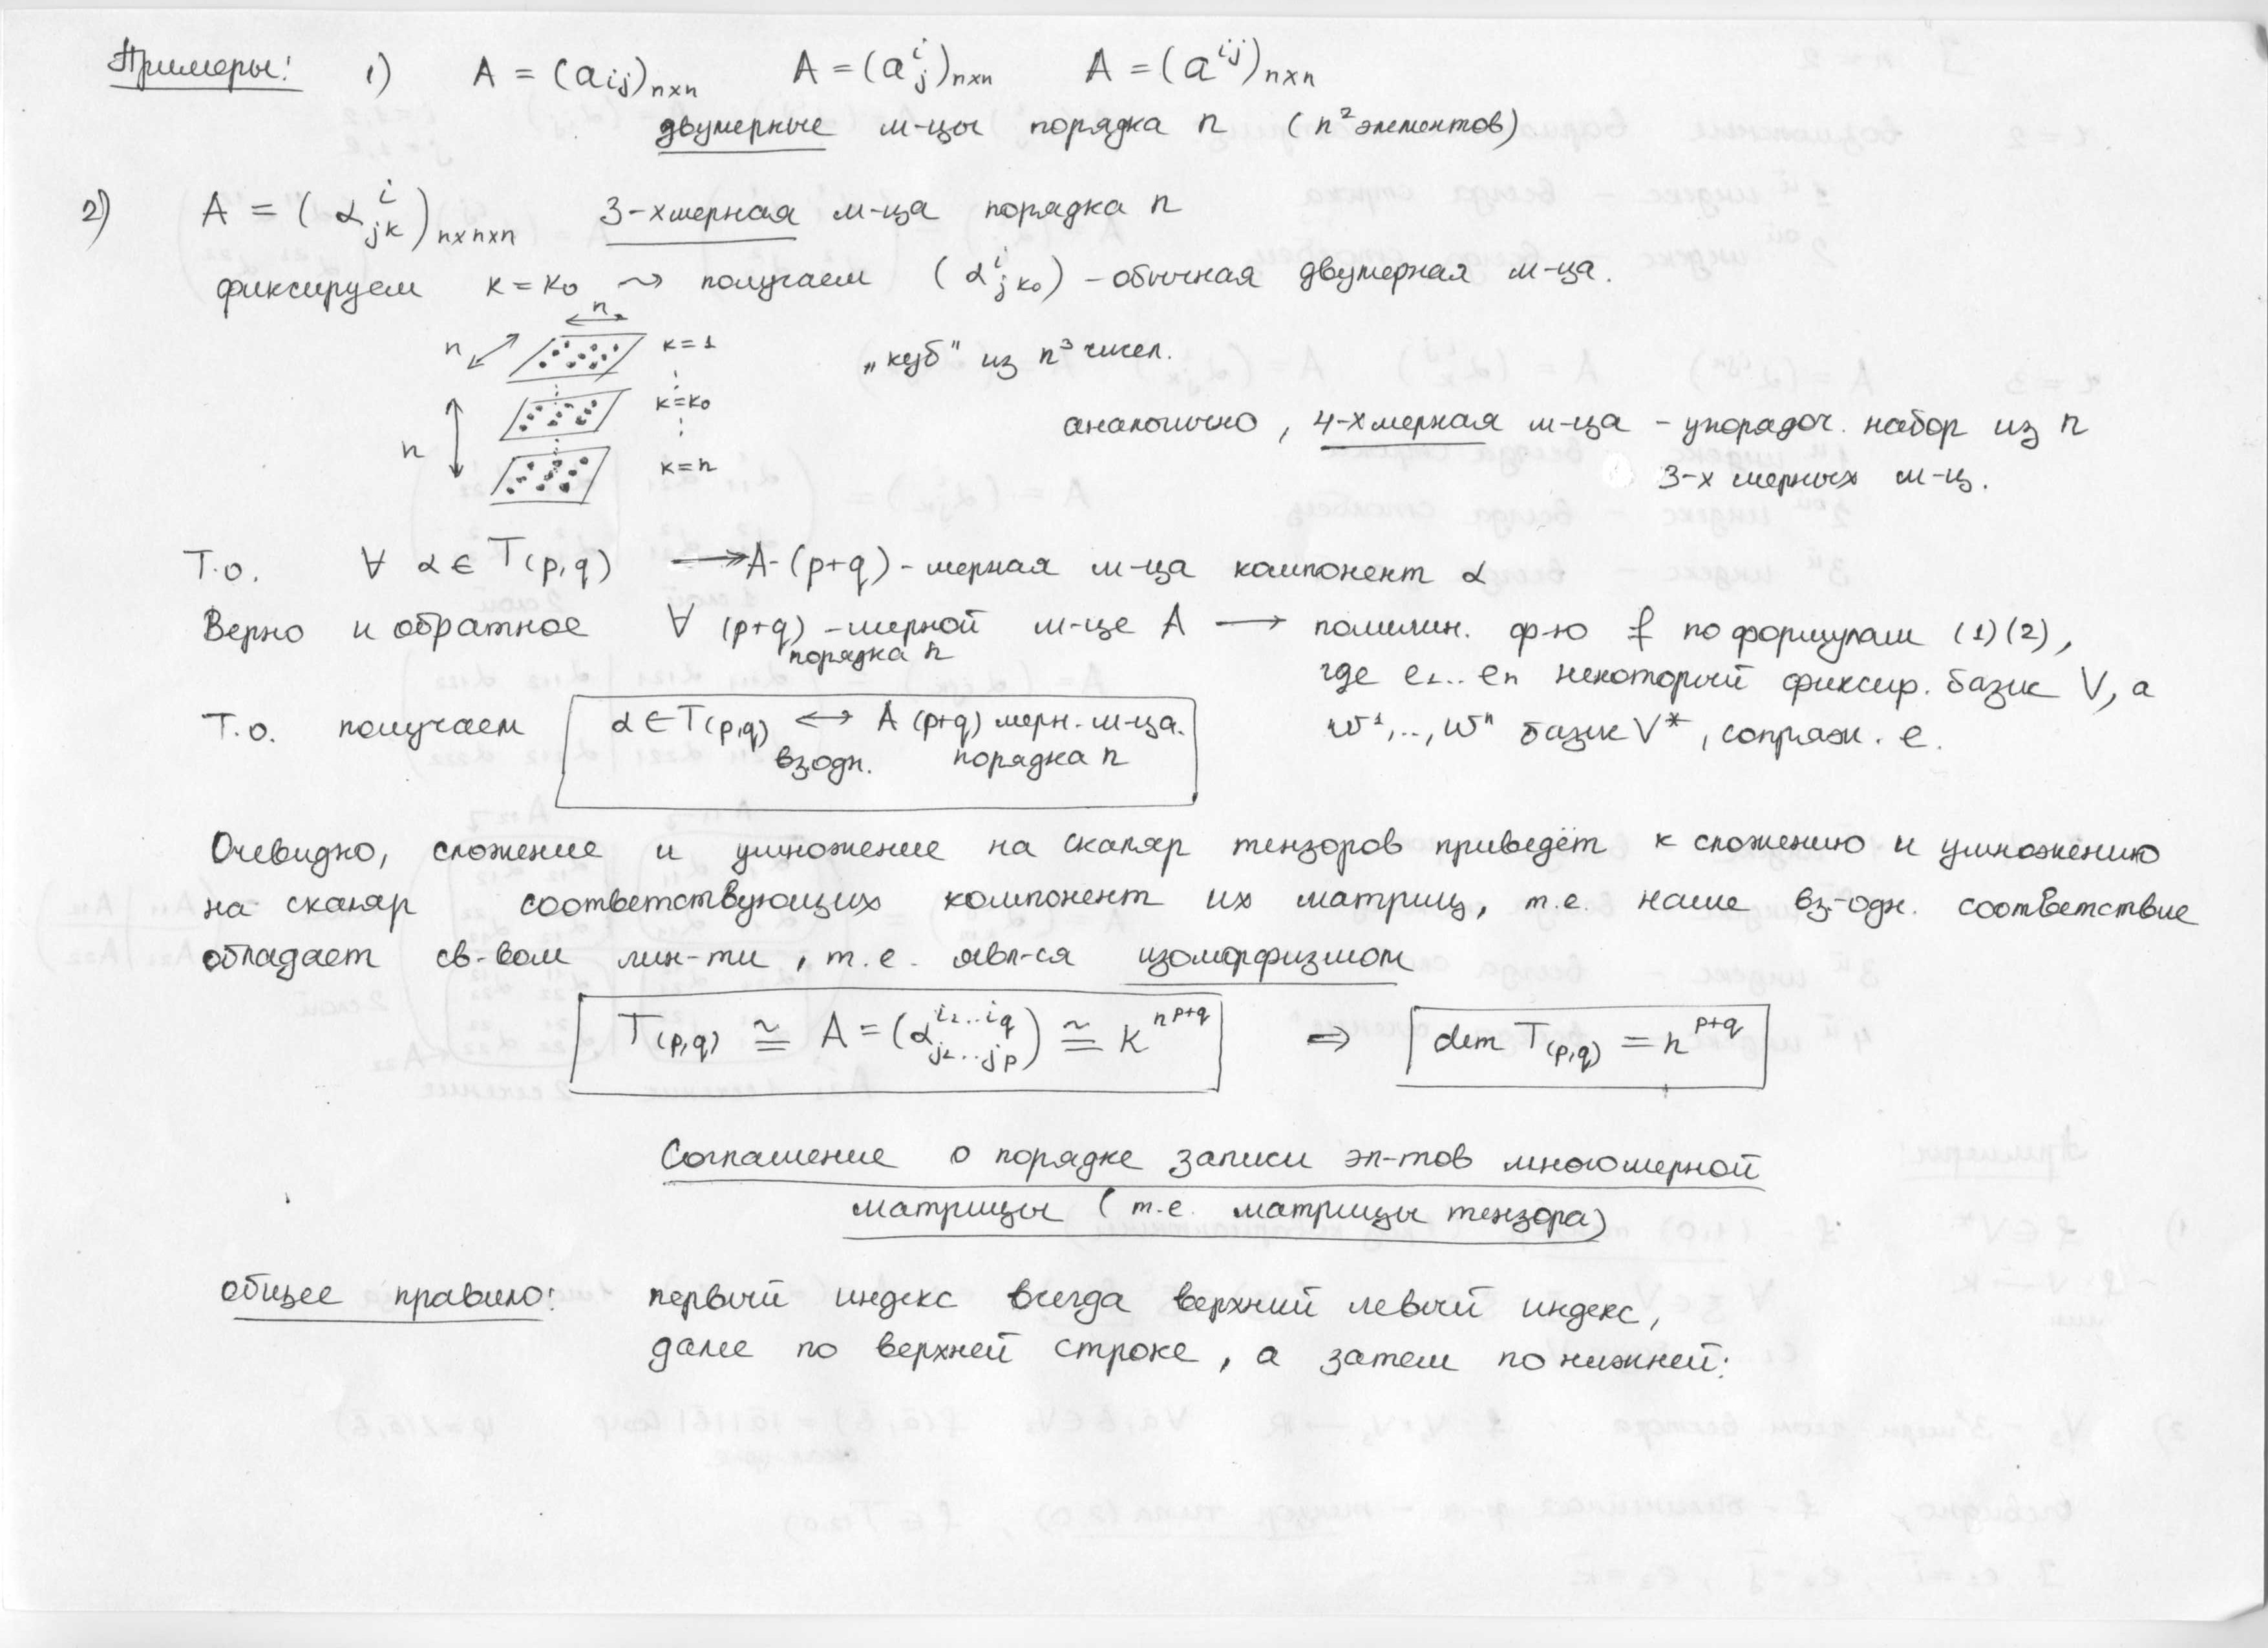
\includegraphics[height=0.49\textheight, width=\textwidth]{8_2-3}	
		\n
		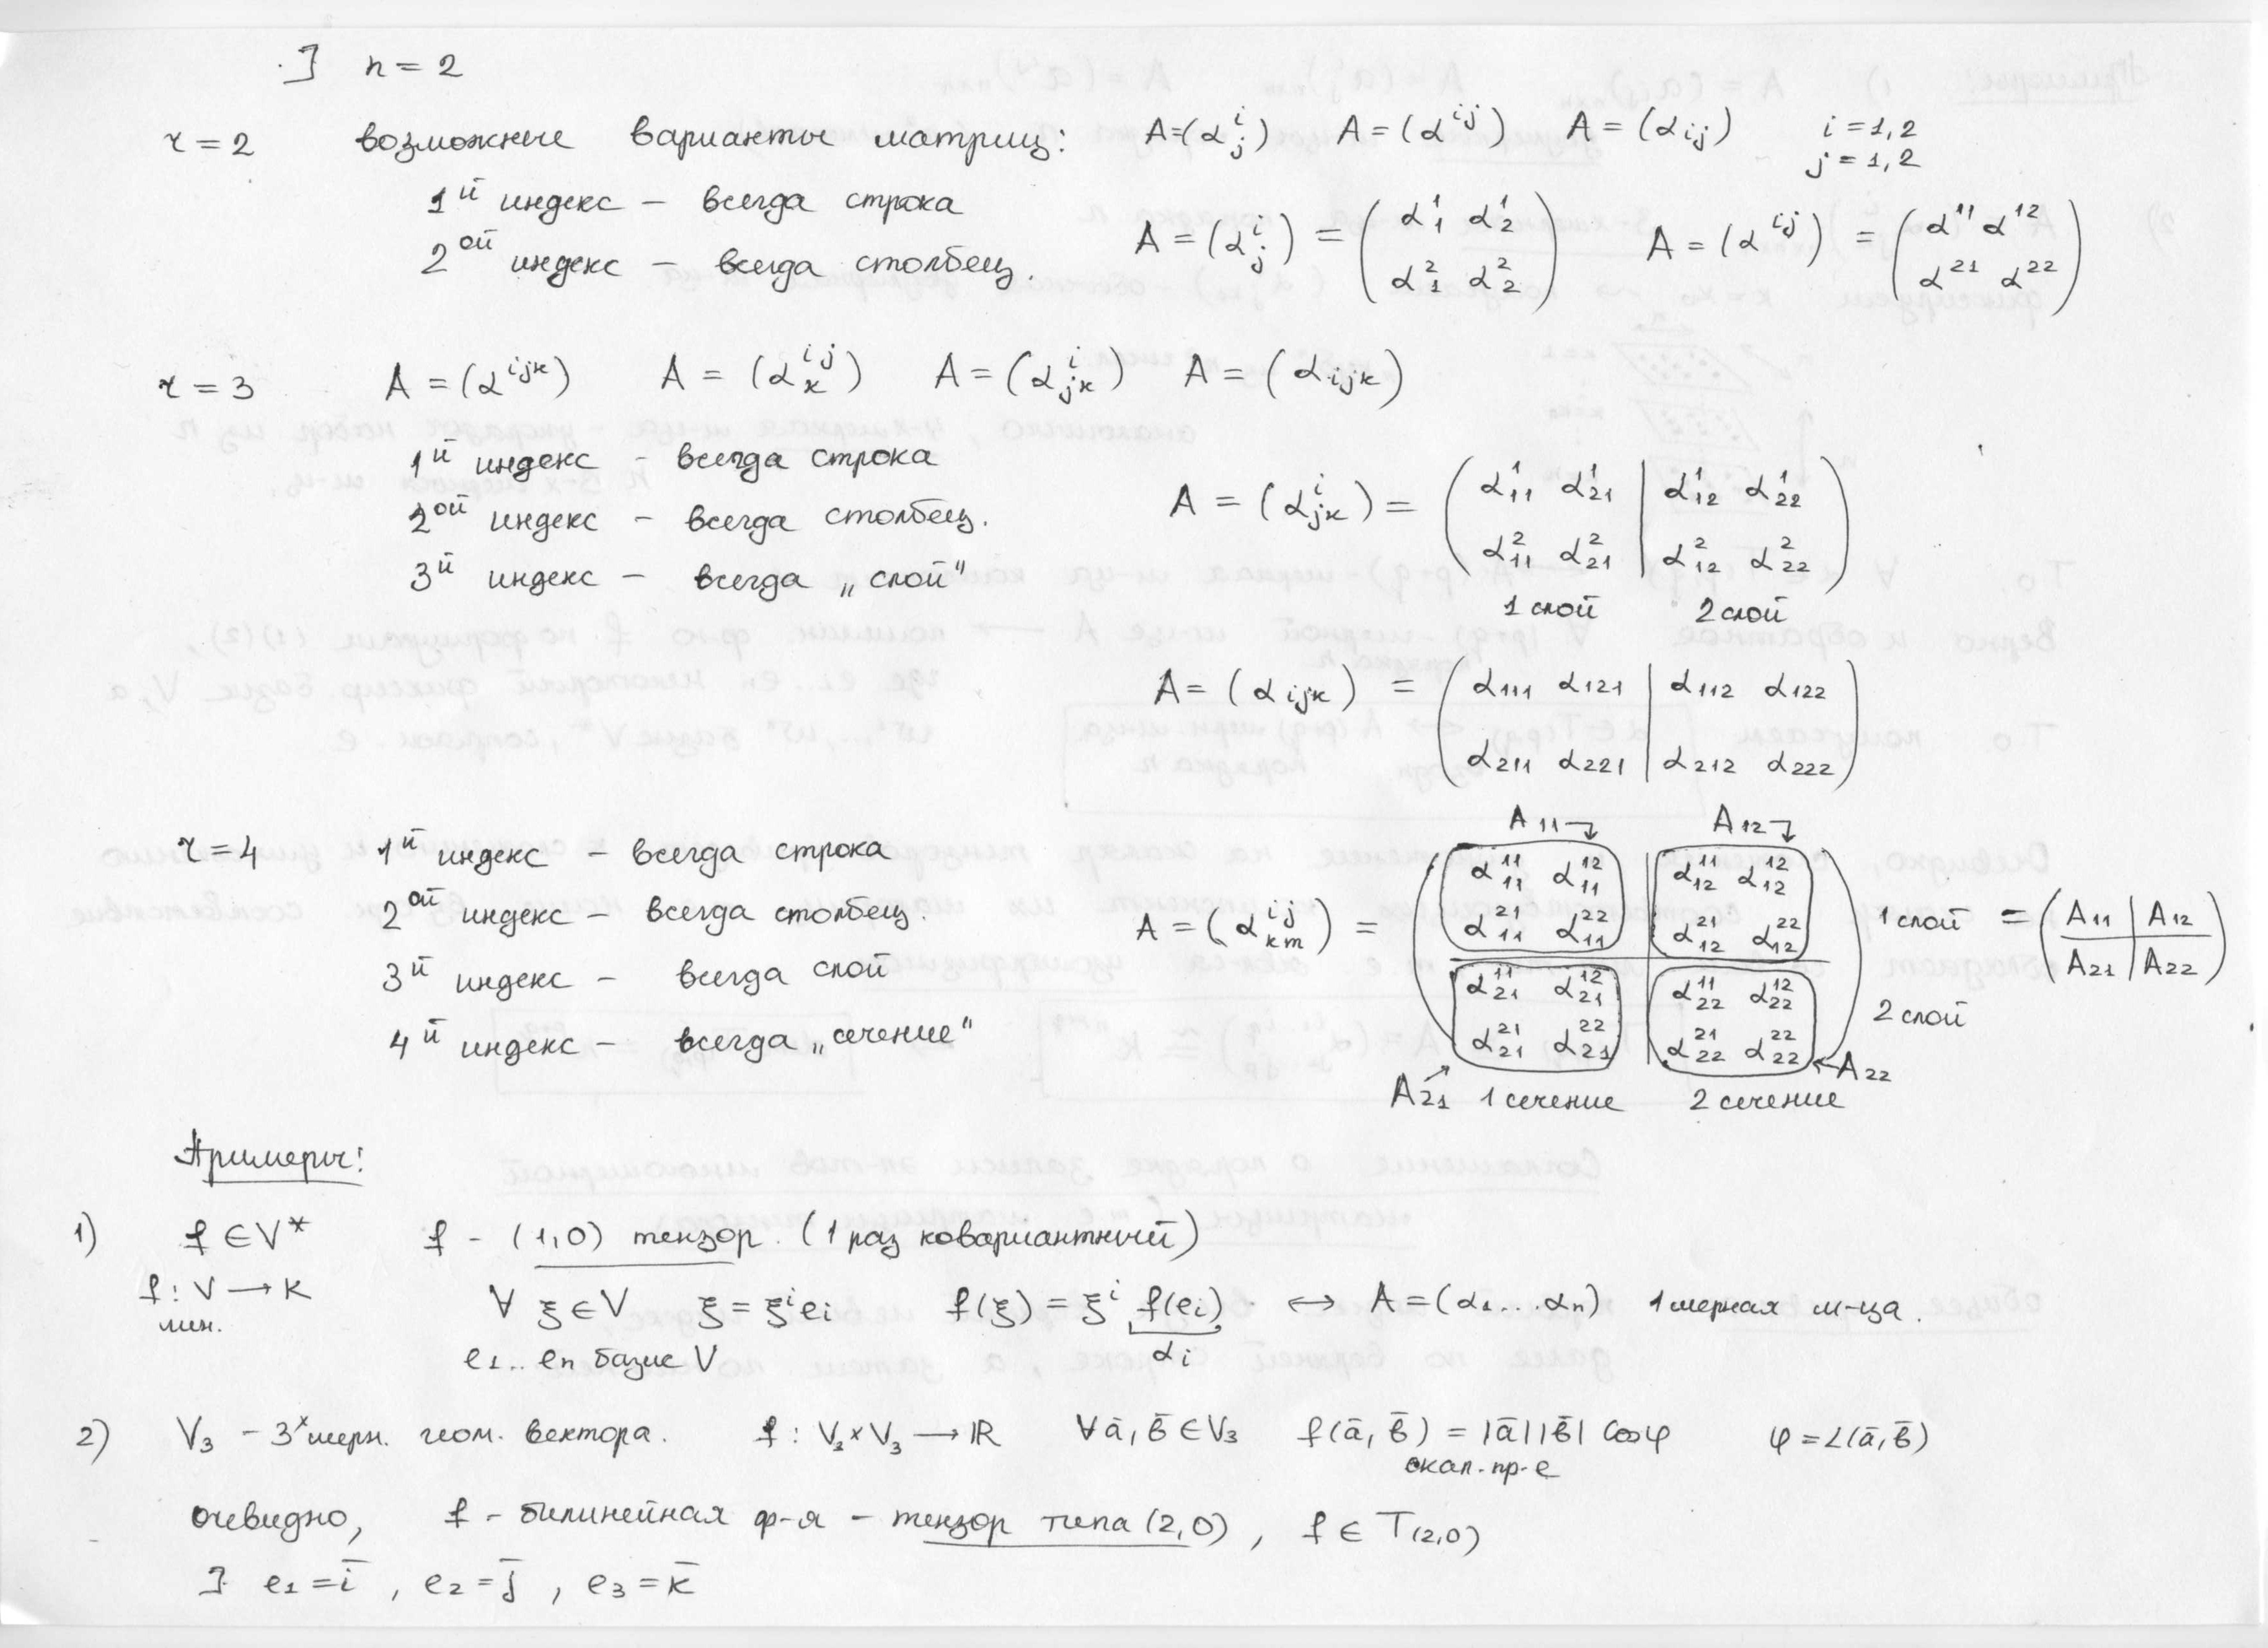
\includegraphics[height=0.49\textheight, width=\textwidth]{8_2-4}	
		\n
		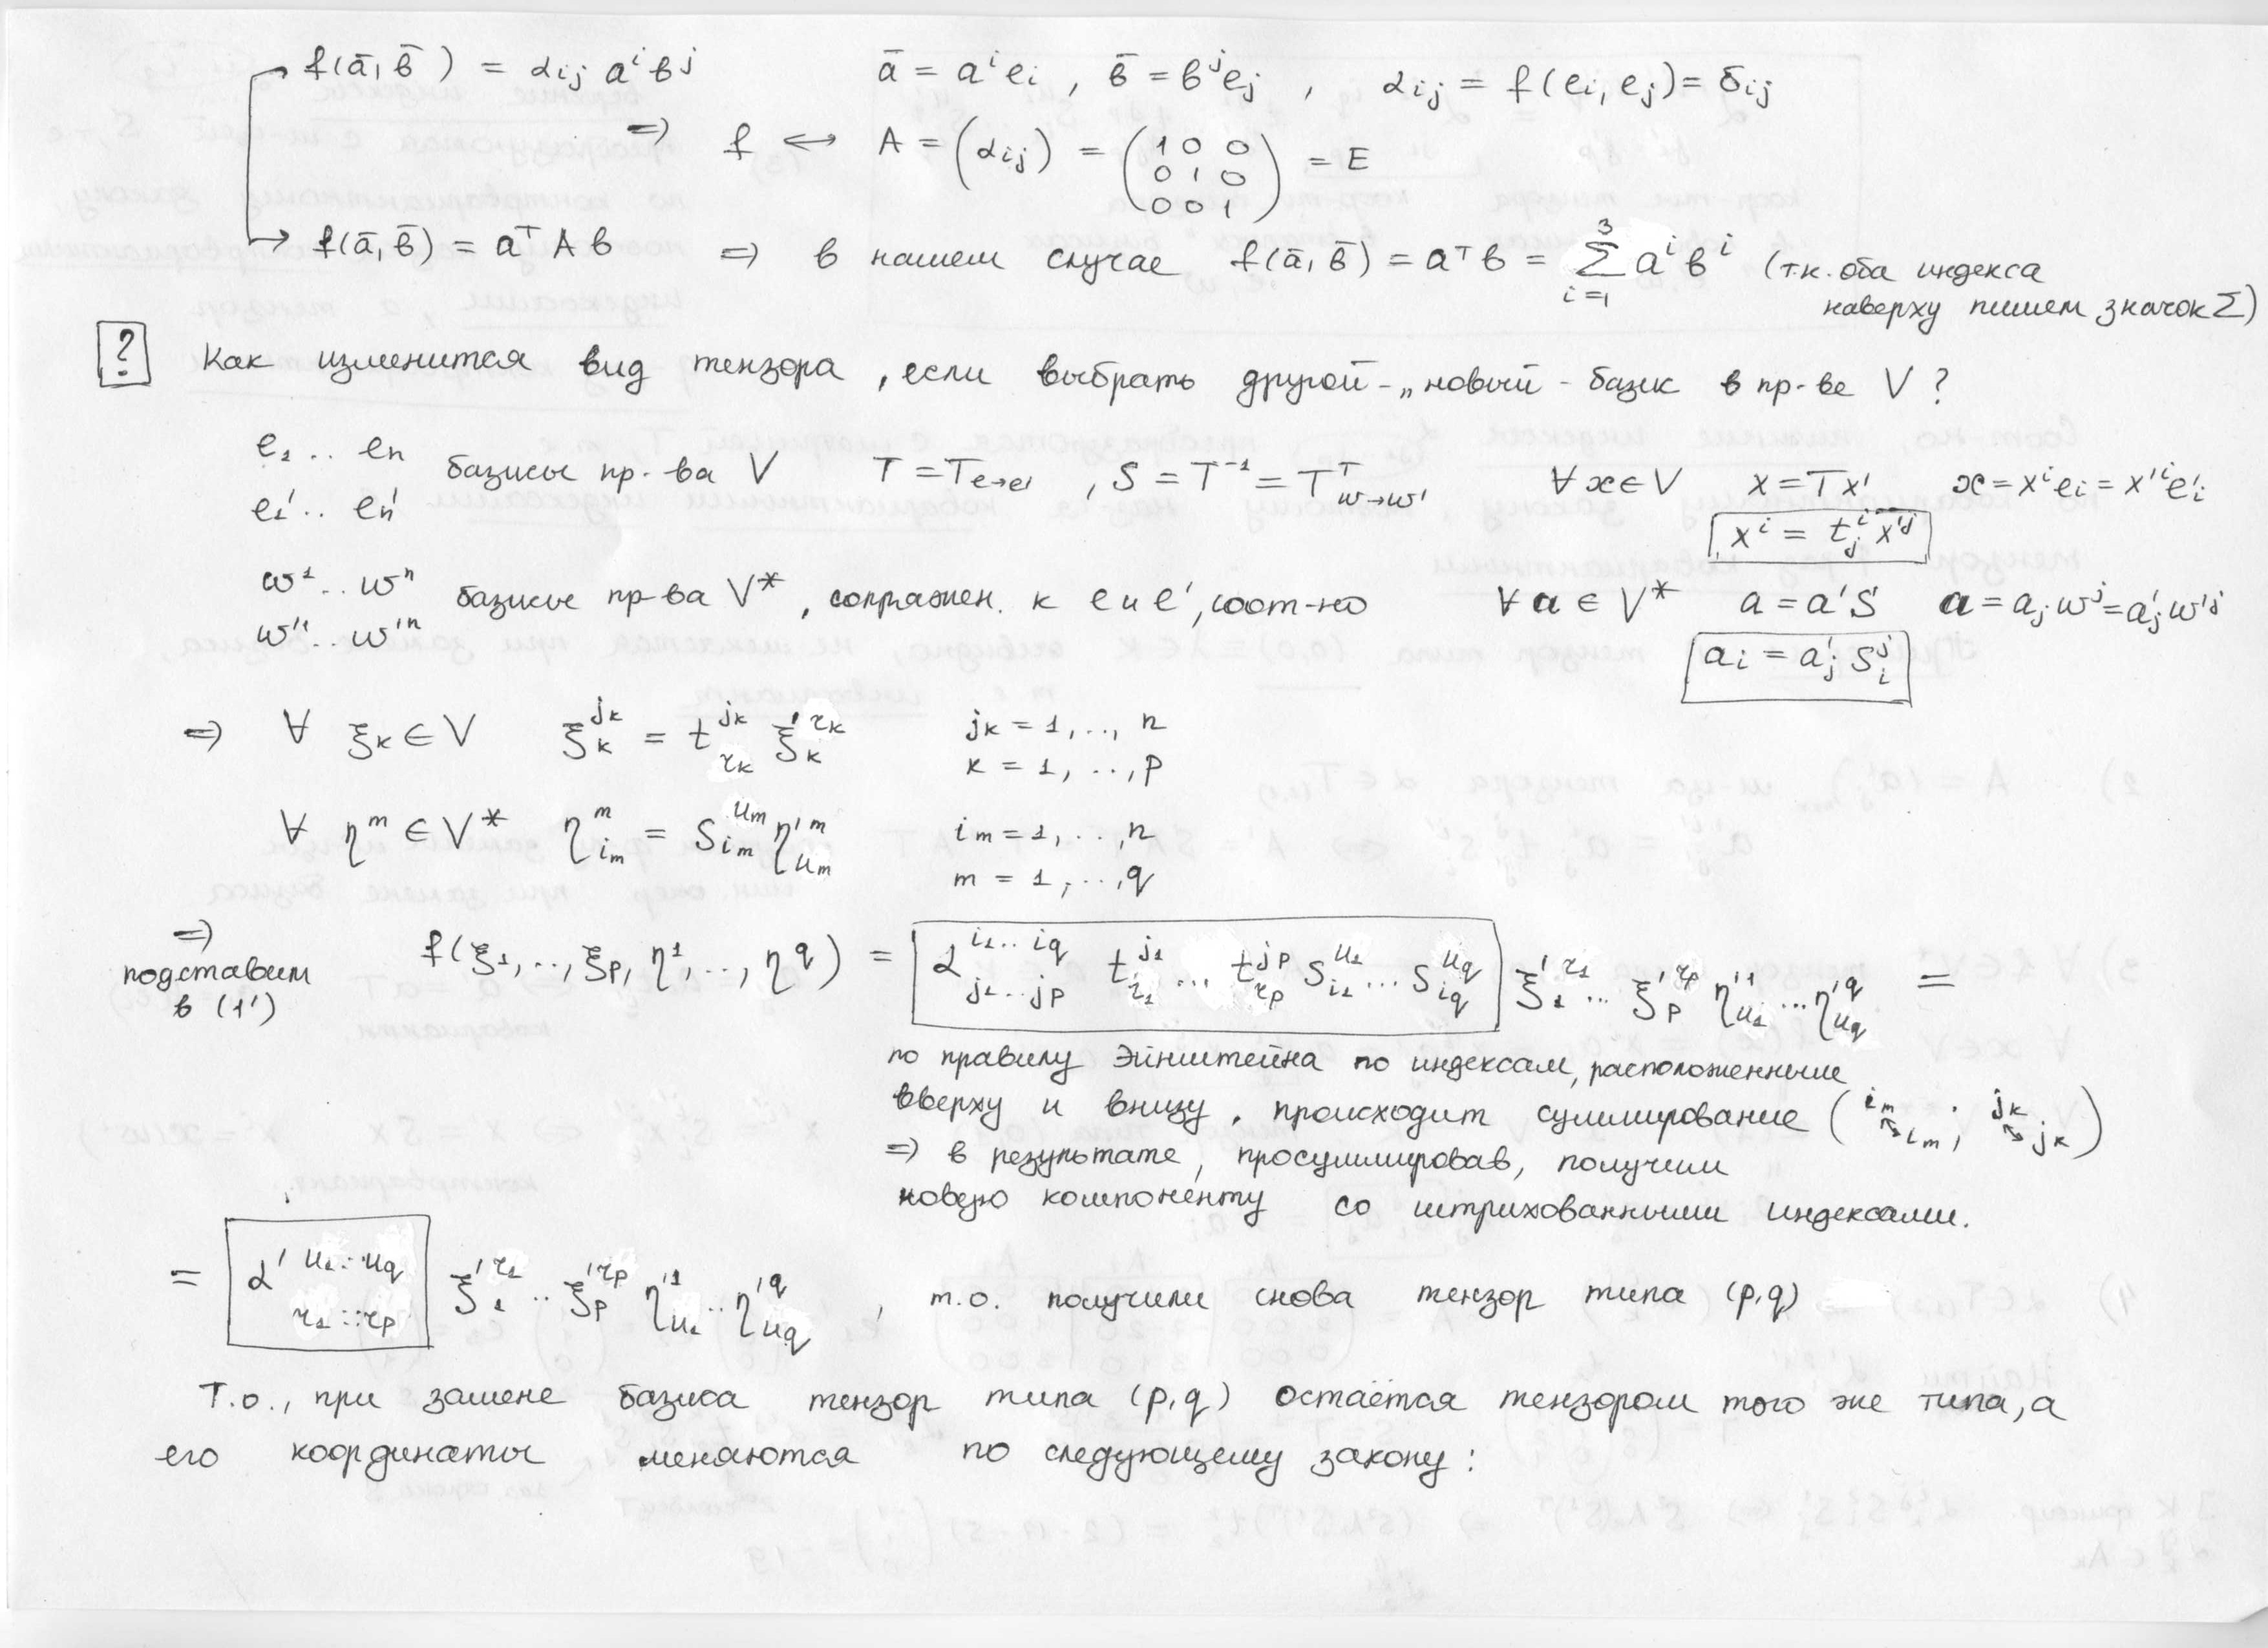
\includegraphics[height=0.49\textheight, width=\textwidth]{8_2-5}	
		\n
		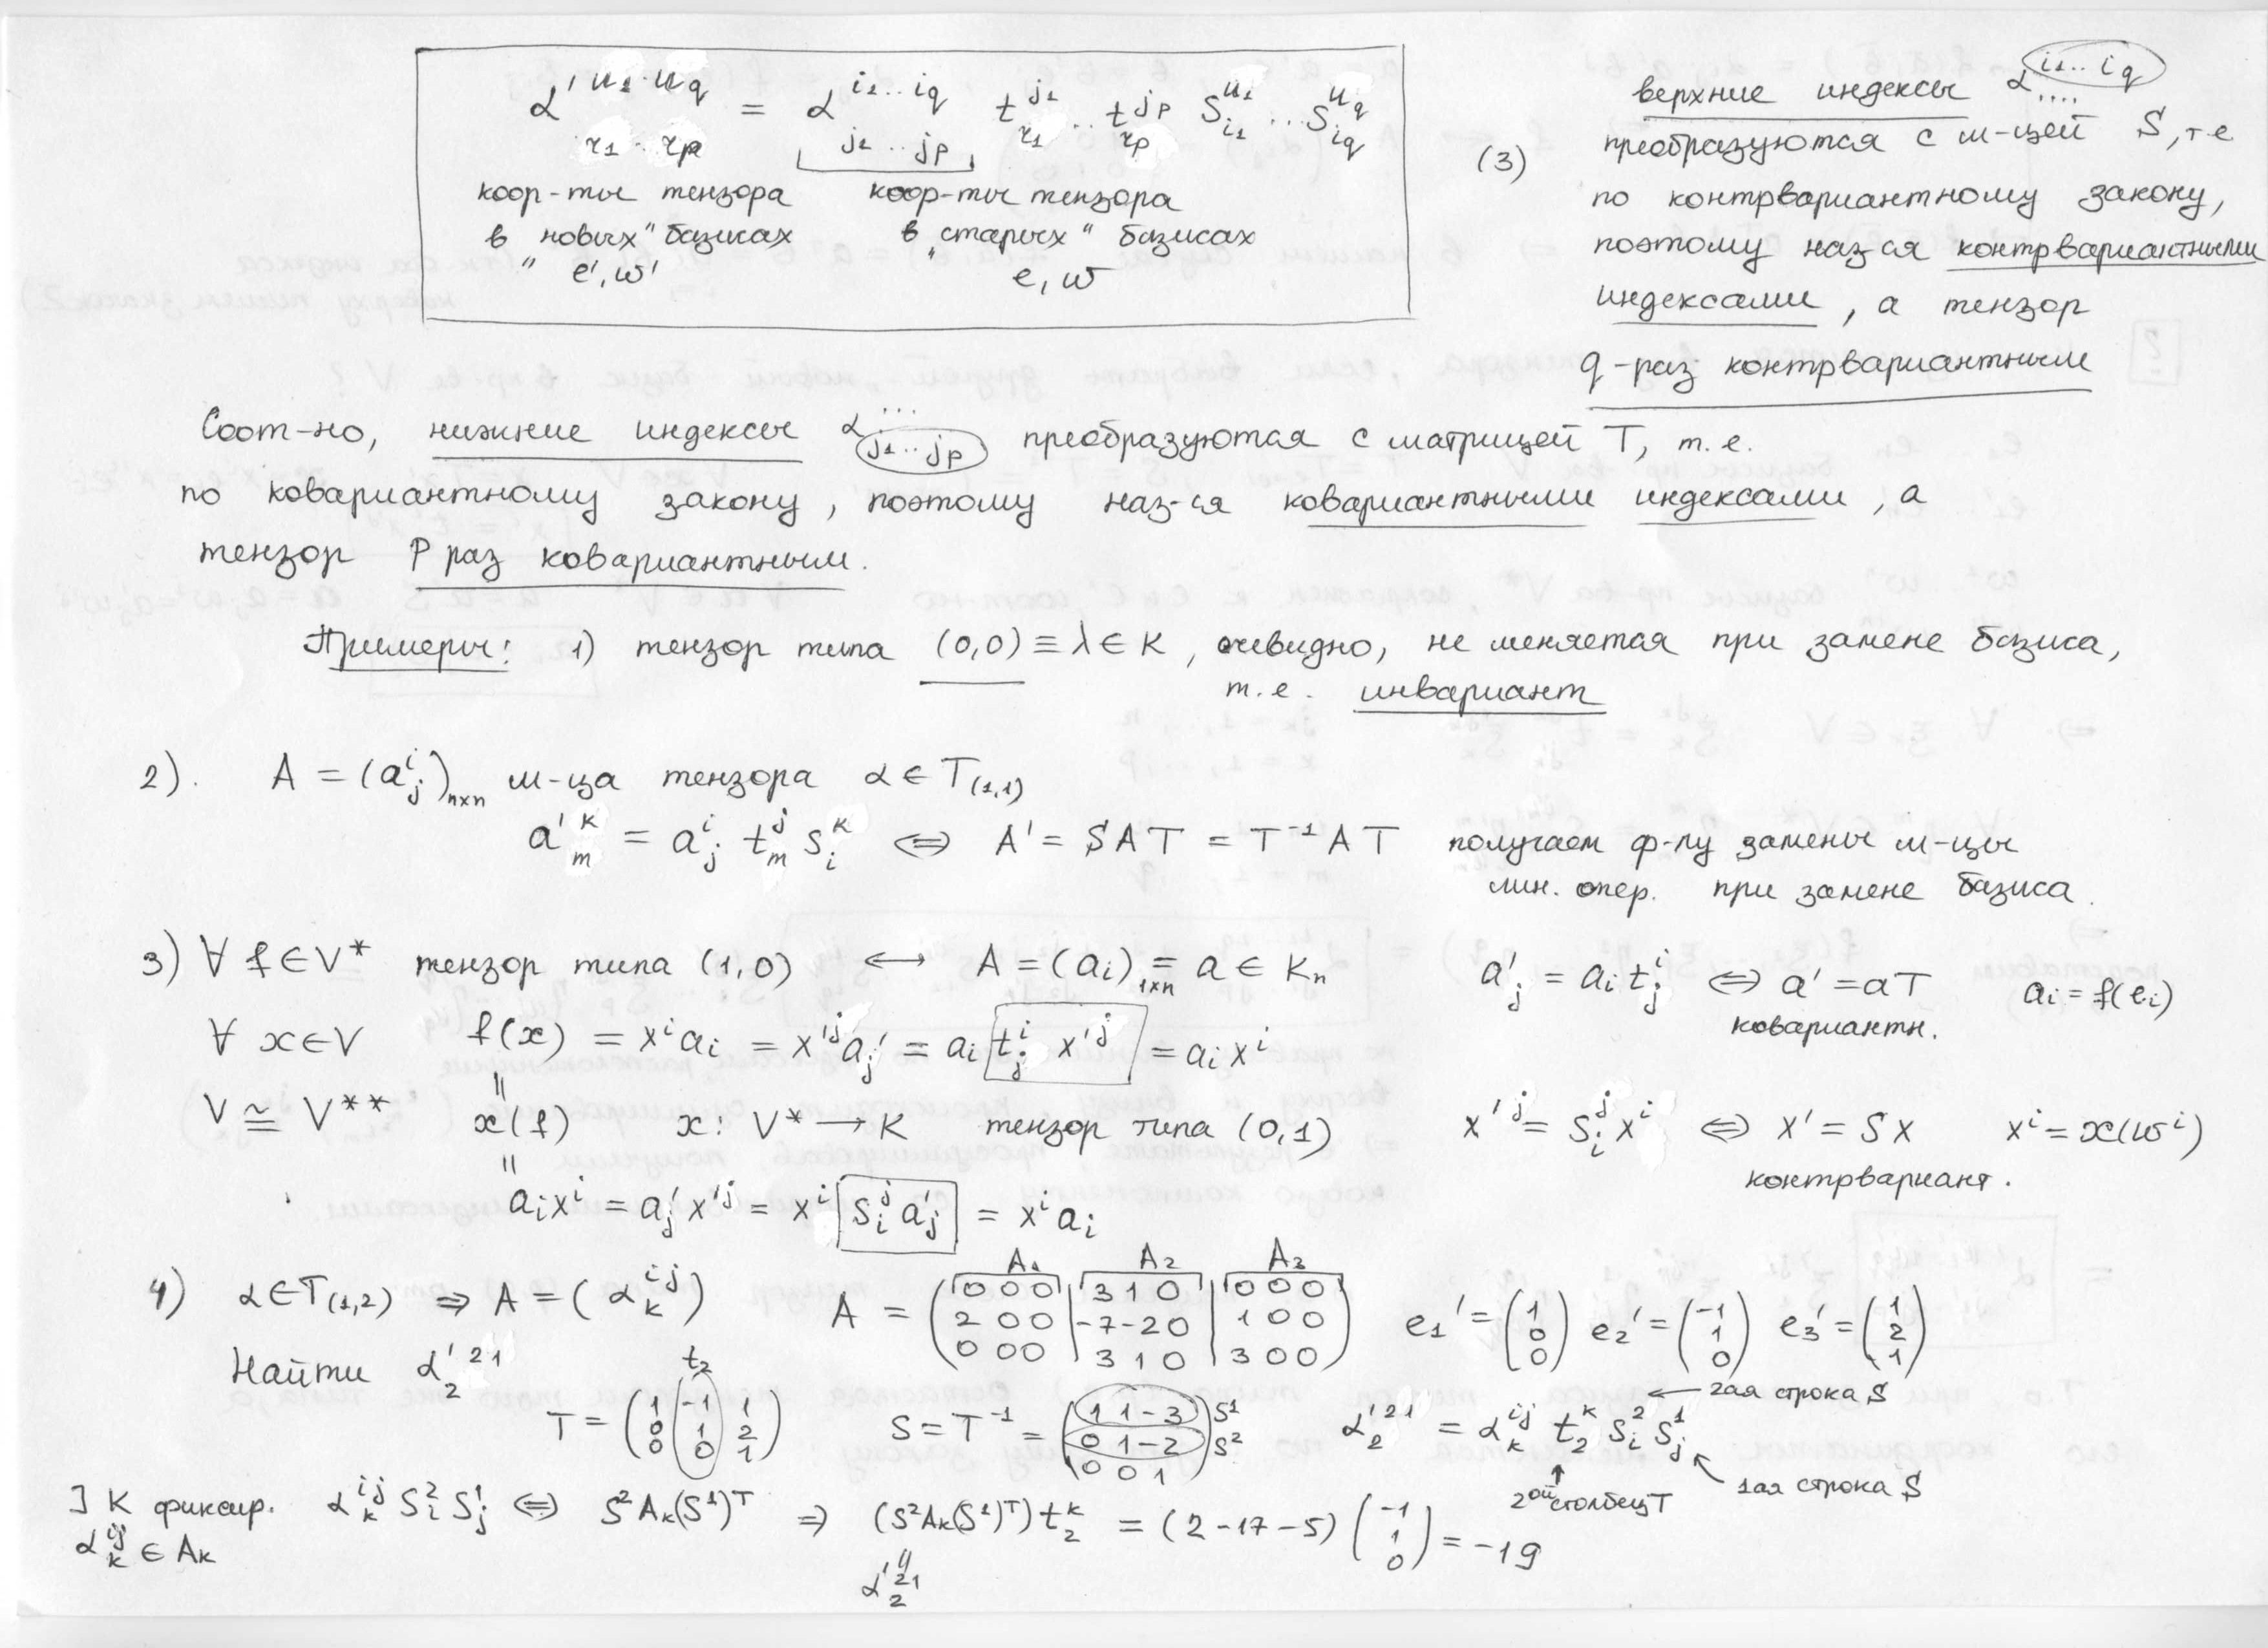
\includegraphics[height=0.49\textheight, width=\textwidth]{8_2-6}	
		\n
		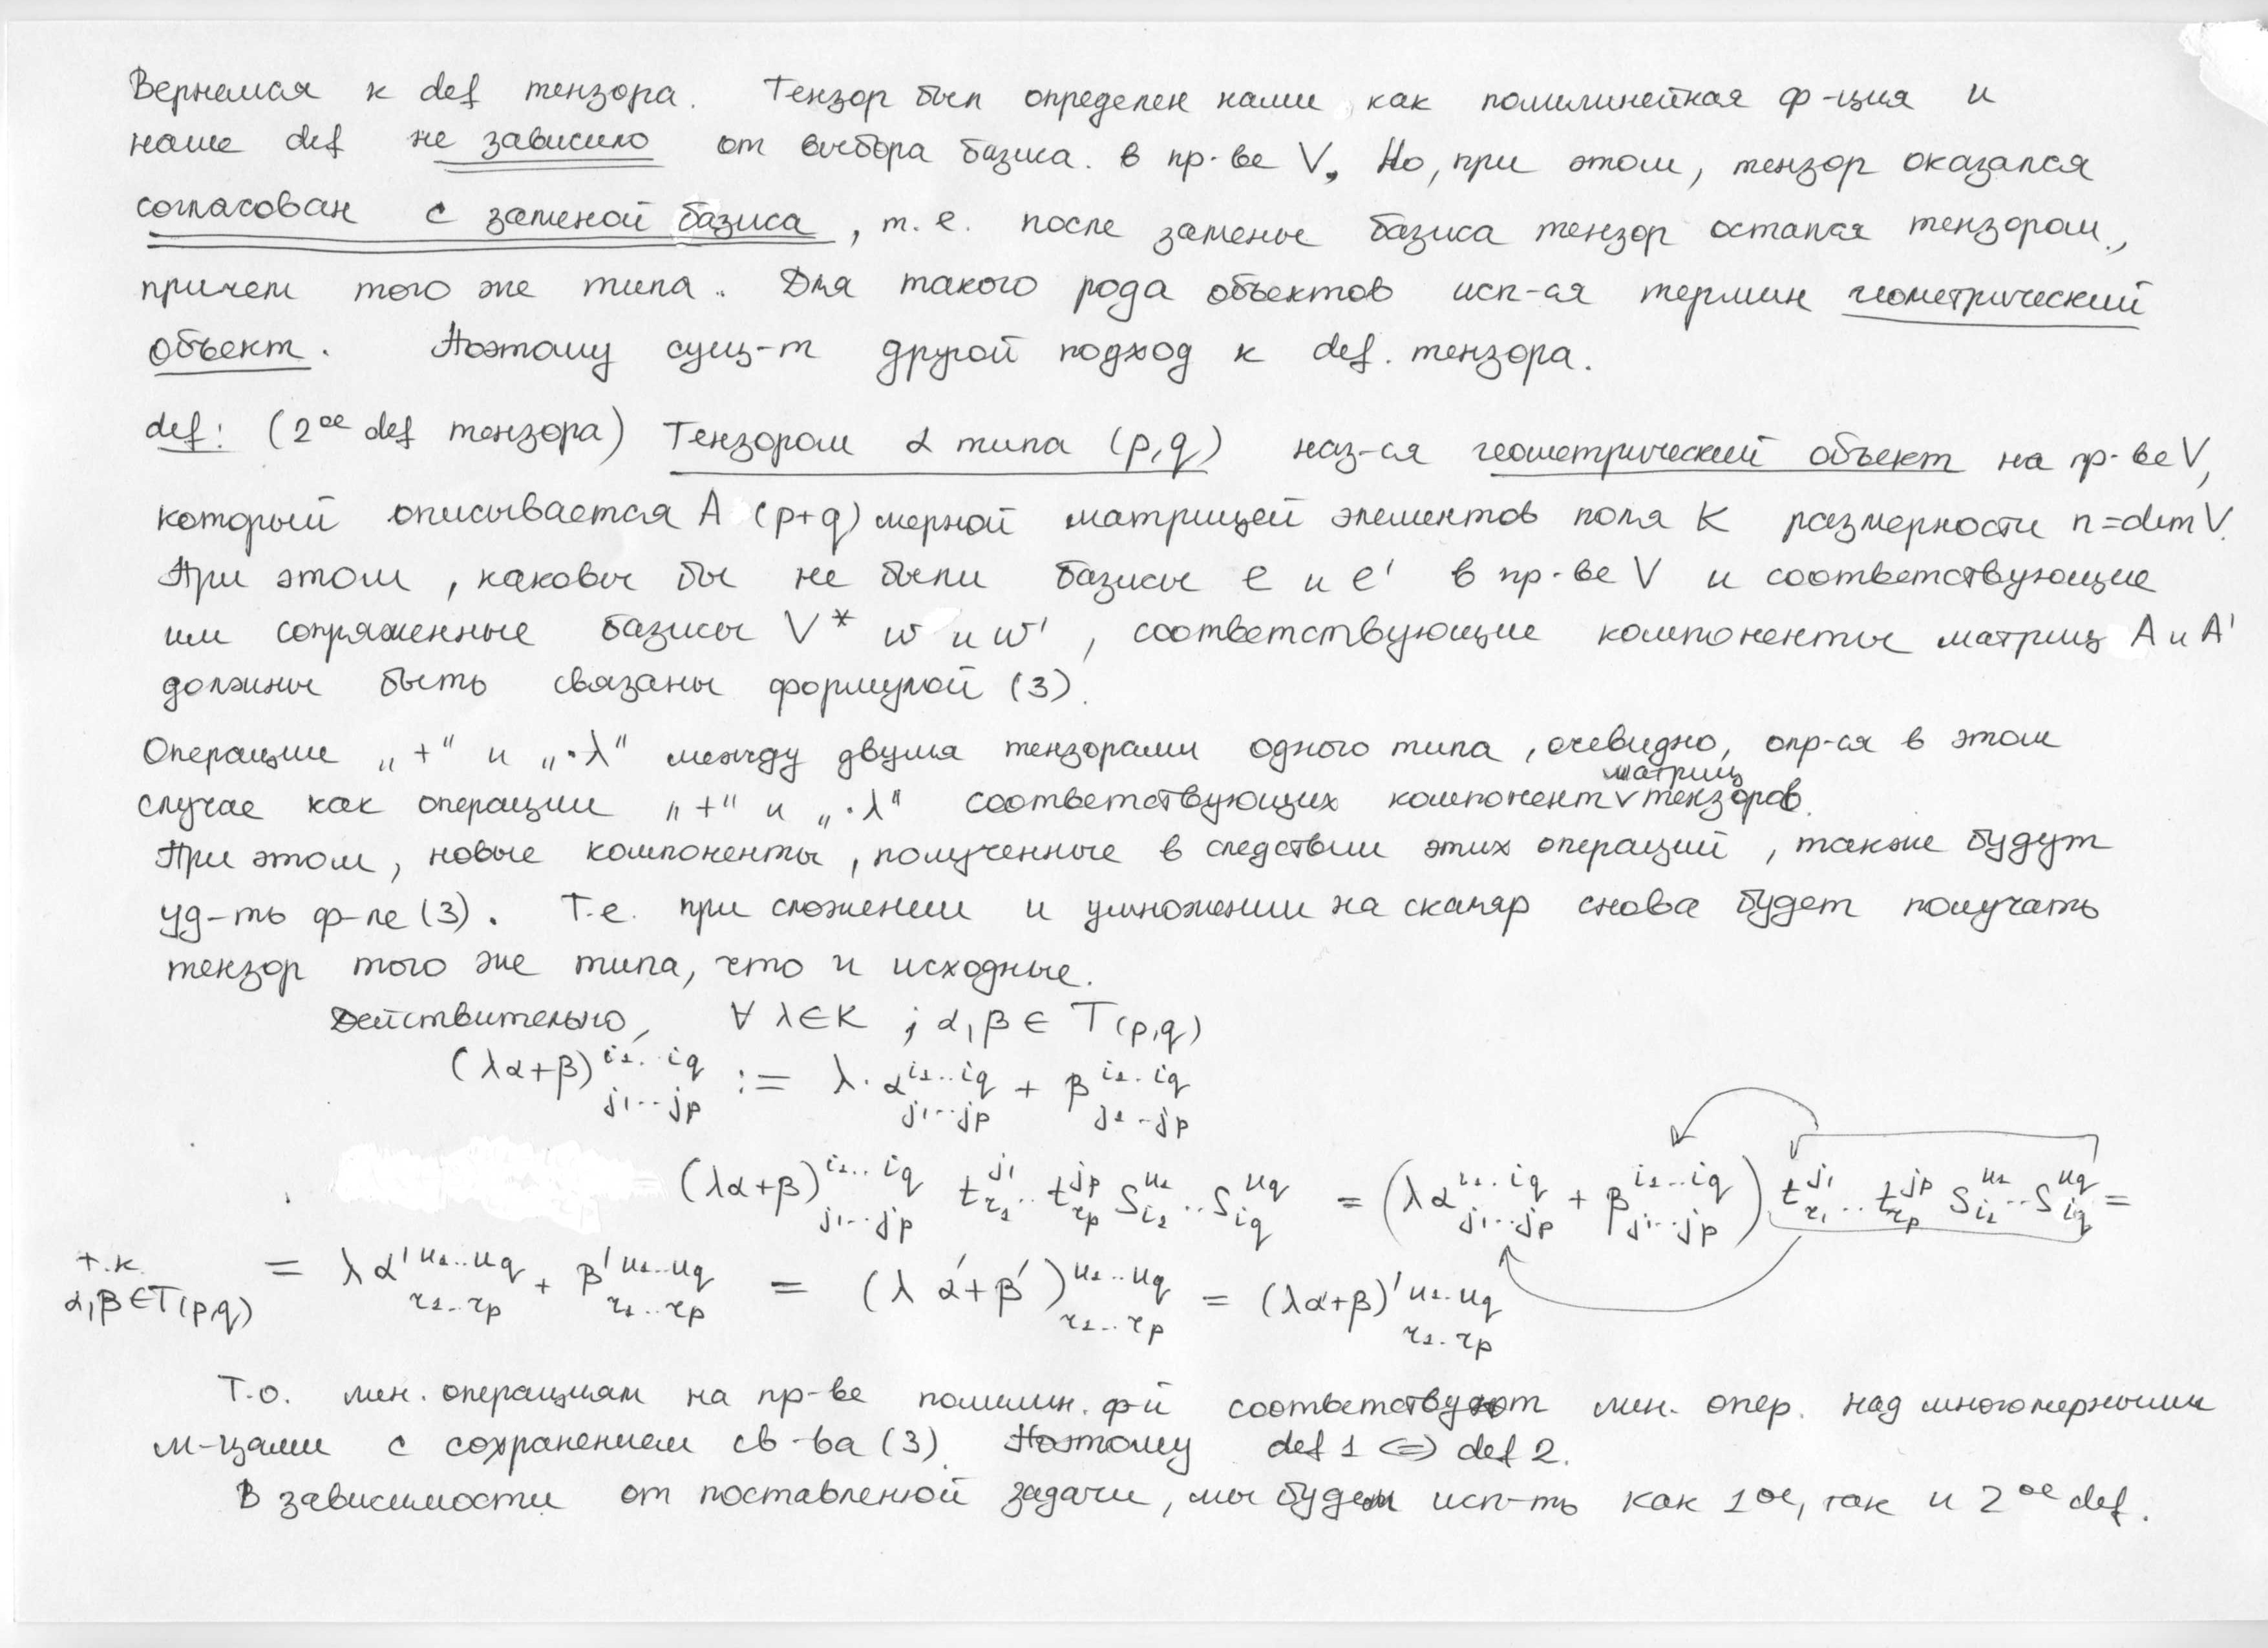
\includegraphics[height=0.49\textheight, width=\textwidth]{8_2-7}	
		
		
	\subsection{Два определения тензора. Многомерная матрица. Линейной пространство тензоров.}
	 		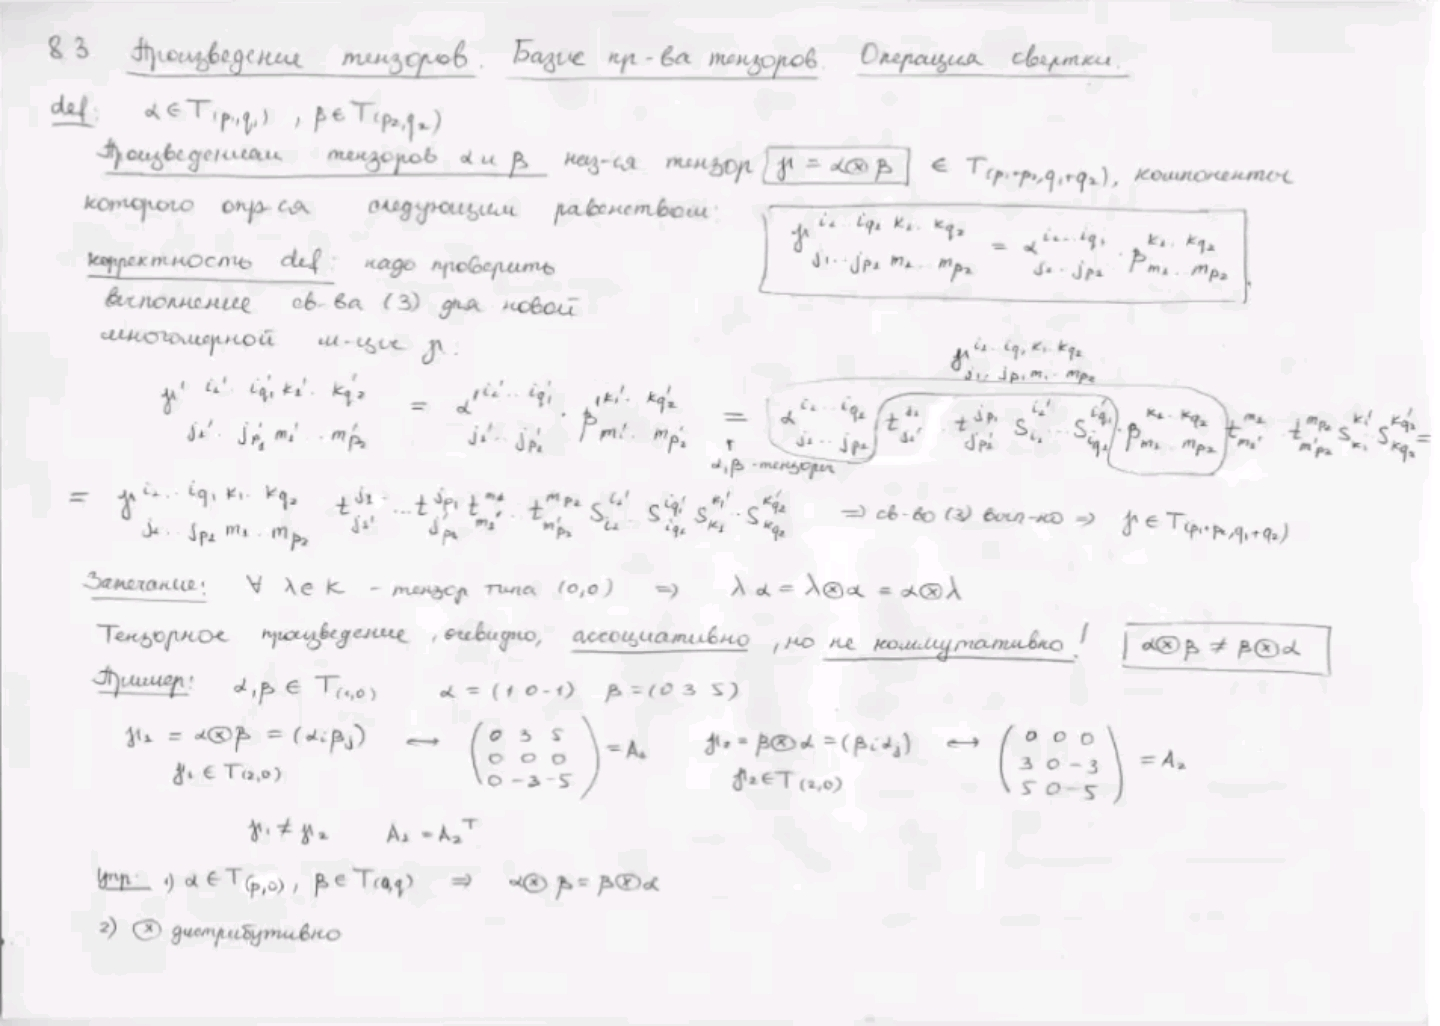
\includegraphics[height=0.49\textheight, width=\textwidth]{new/New_00001}	
		\n
		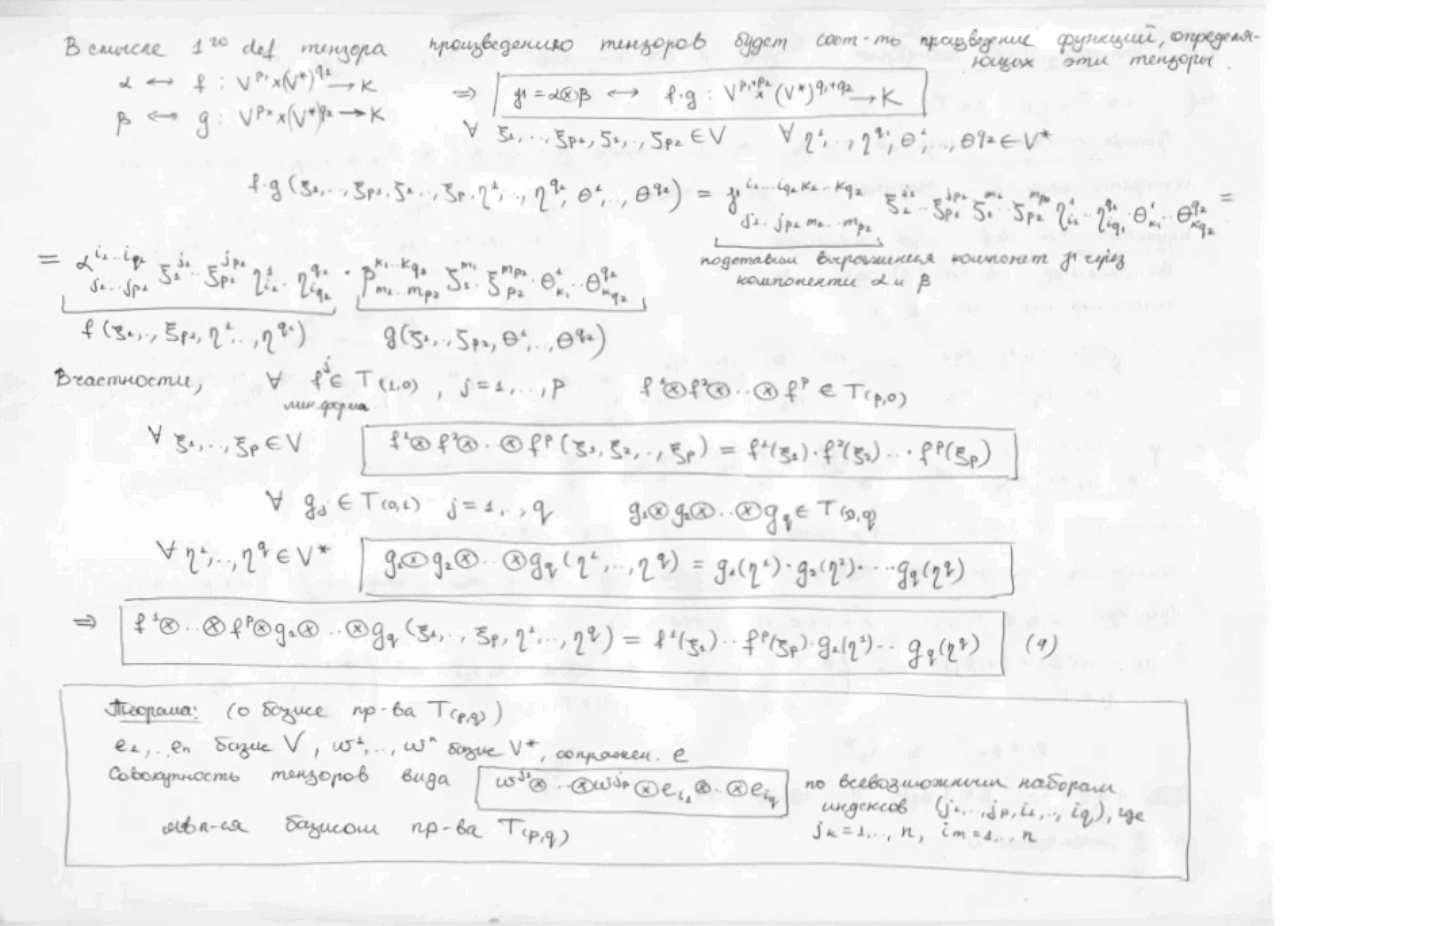
\includegraphics[height=0.49\textheight, width=\textwidth]{new/New_00002}	
		\n
		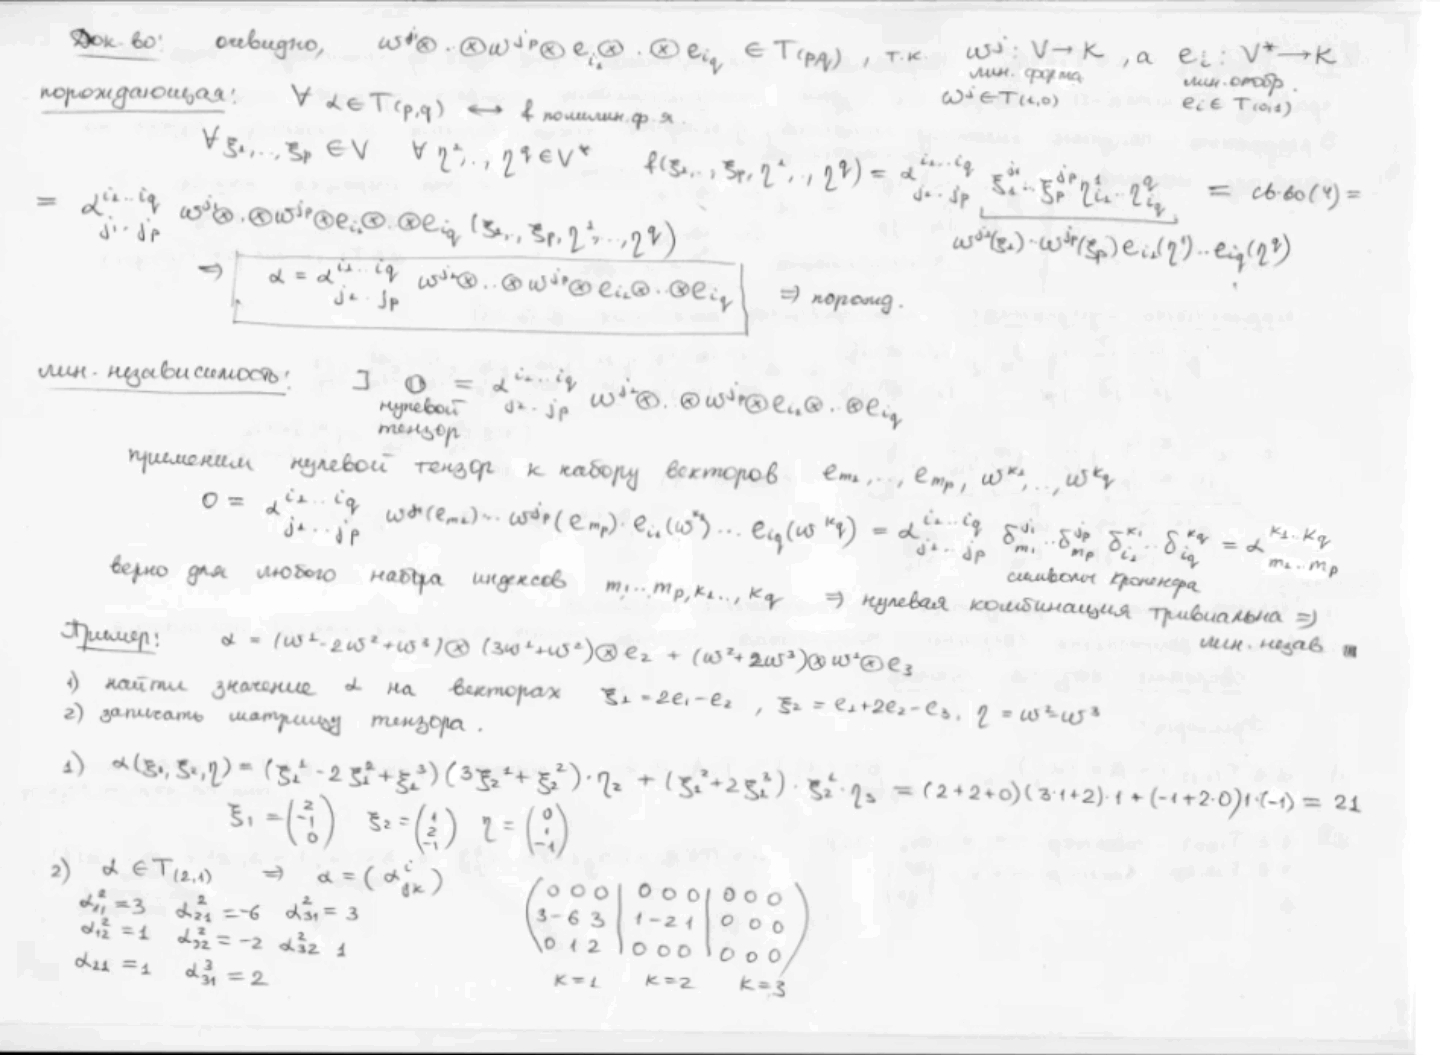
\includegraphics[height=0.49\textheight, width=\textwidth]{new/New_00003}		
		\n
		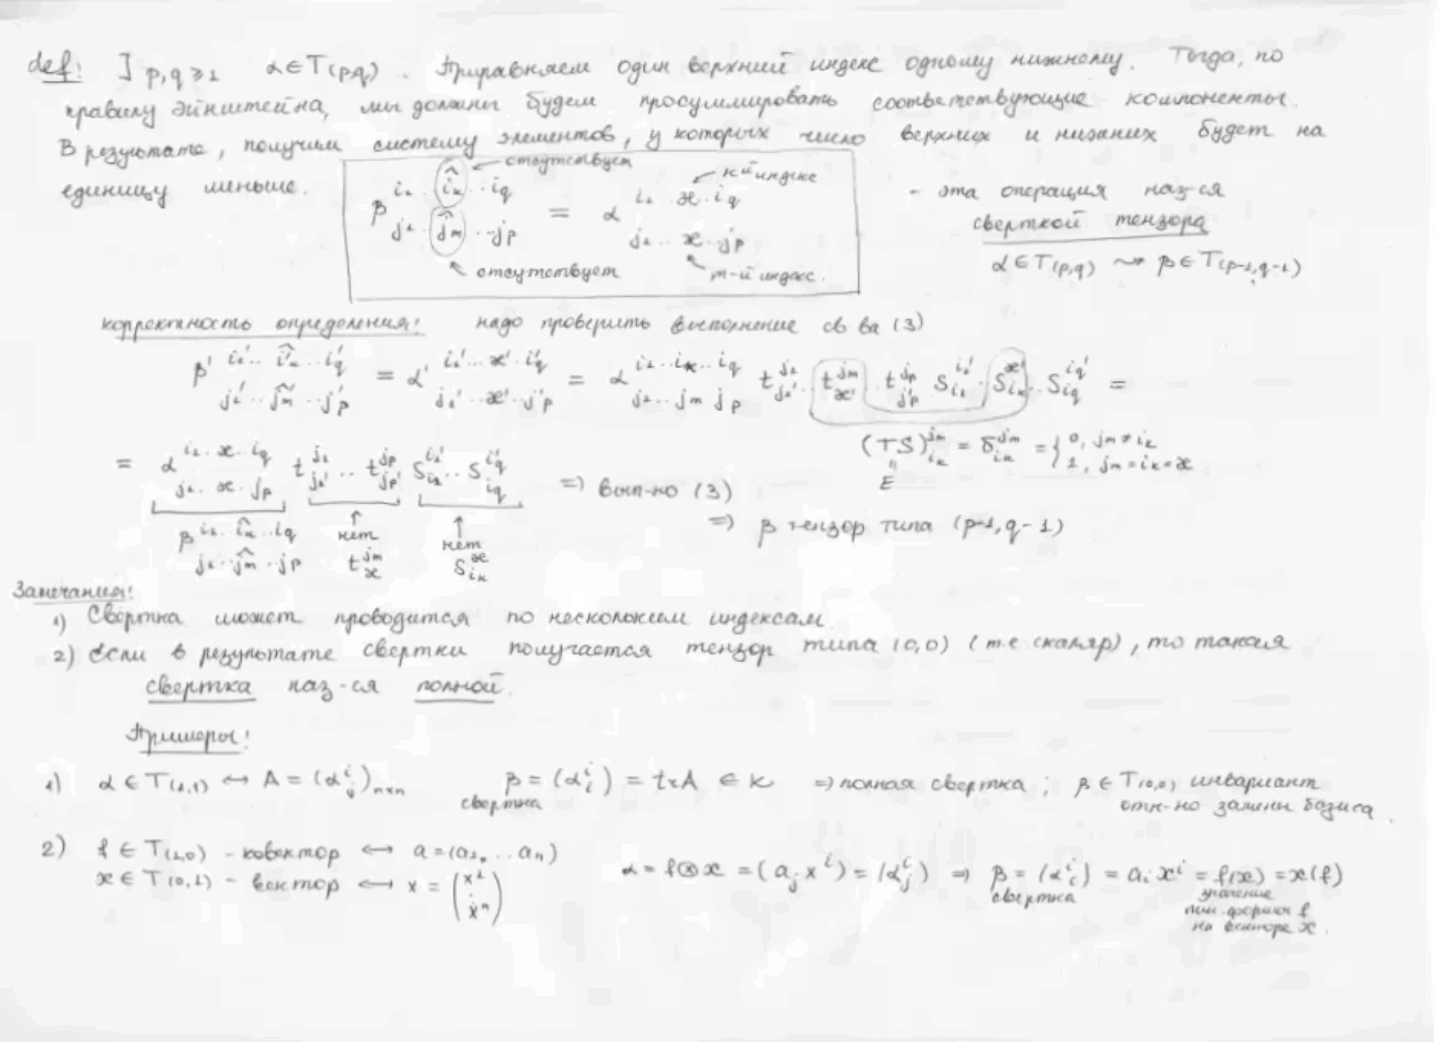
\includegraphics[height=0.49\textheight, width=\textwidth]{new/New_00004}	
		\n
		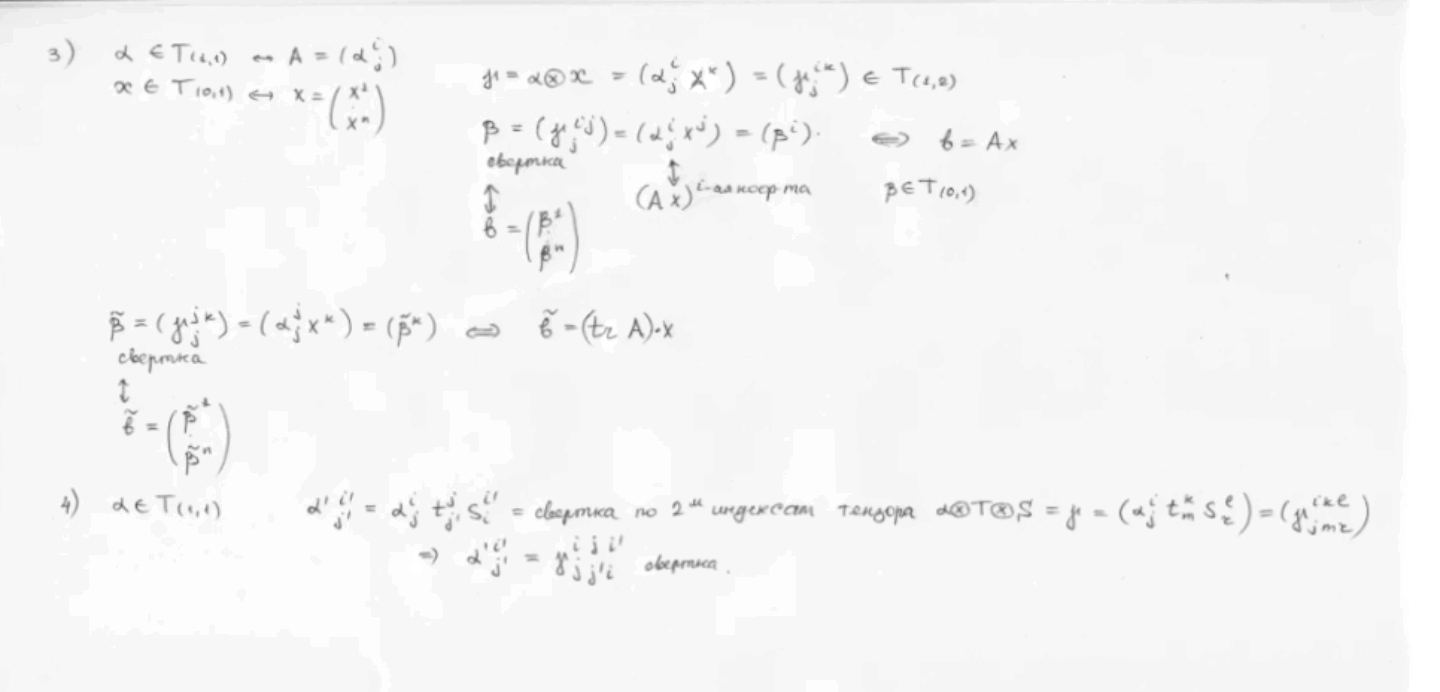
\includegraphics[height=0.49\textheight, width=\textwidth]{new/New_00005}	
		\n			
		
		
	\subsection{Транспонирование тензора. Симметрические и кососимметричческие тензоры.}
	 	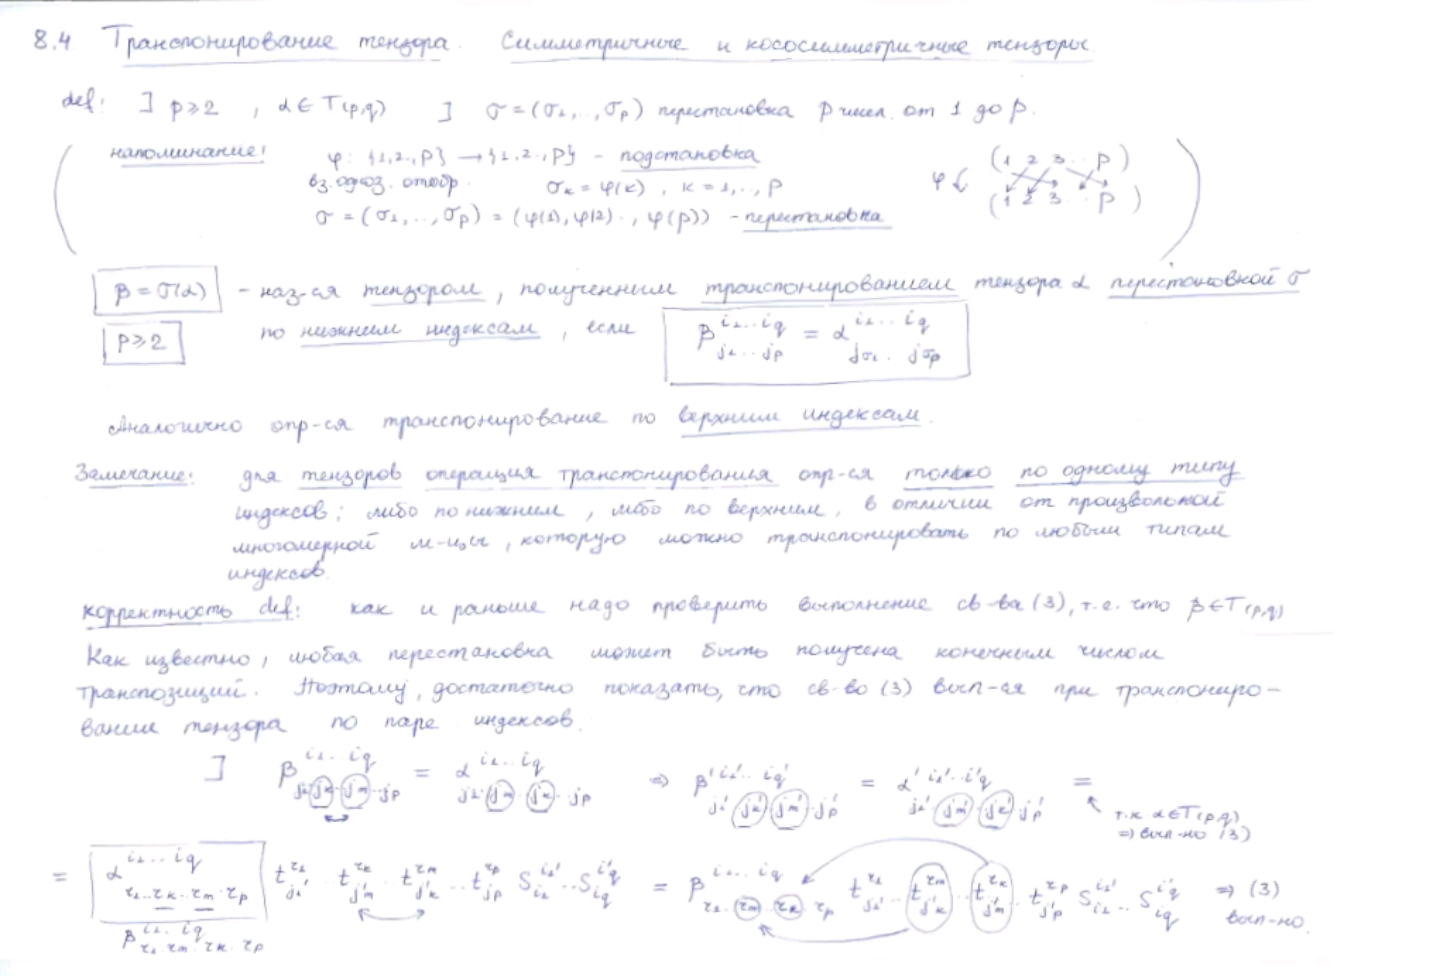
\includegraphics[height=0.49\textheight, width=\textwidth]{new/New_00006}	
		\n
		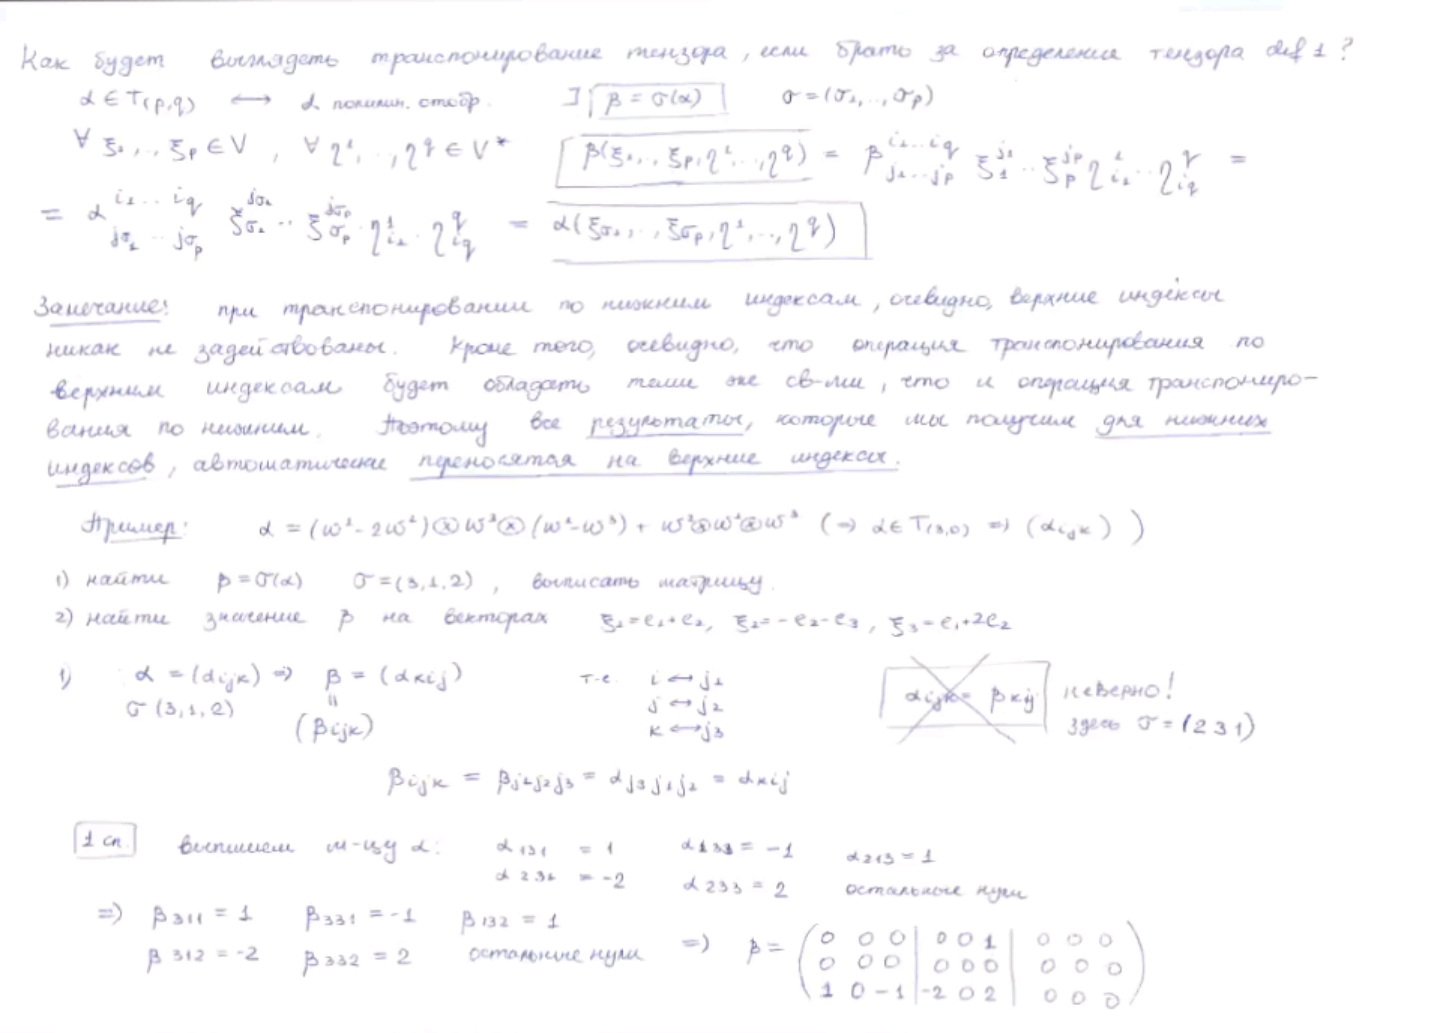
\includegraphics[height=0.49\textheight, width=\textwidth]{new/New_00007}	
		\n
		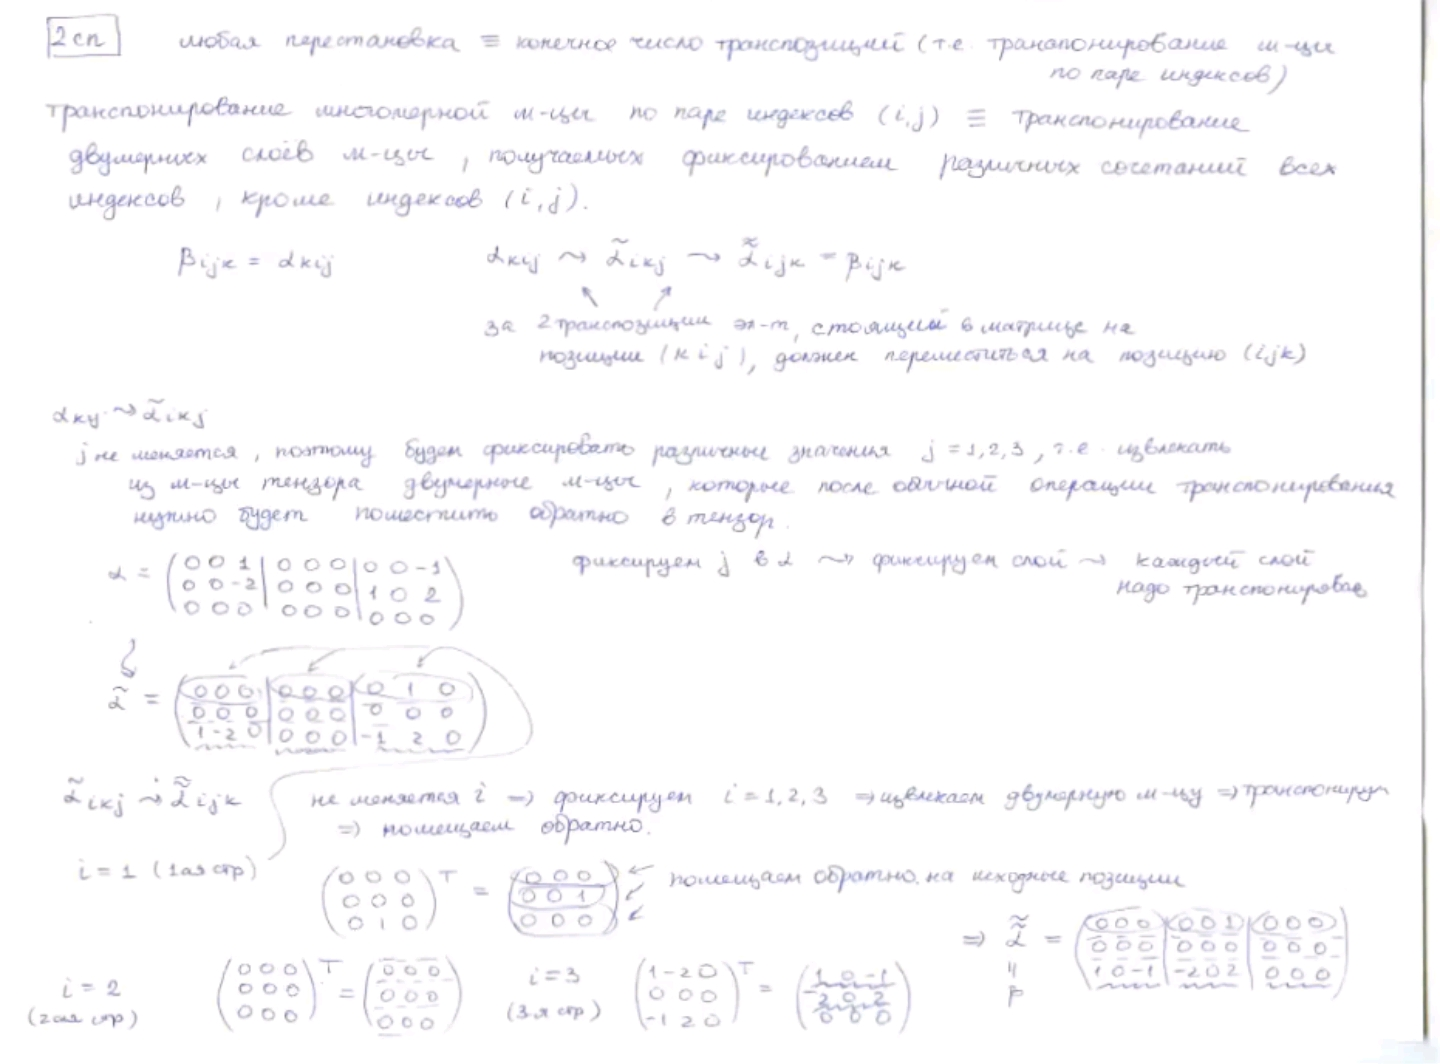
\includegraphics[height=0.49\textheight, width=\textwidth]{new/New_00008}	
		\n
		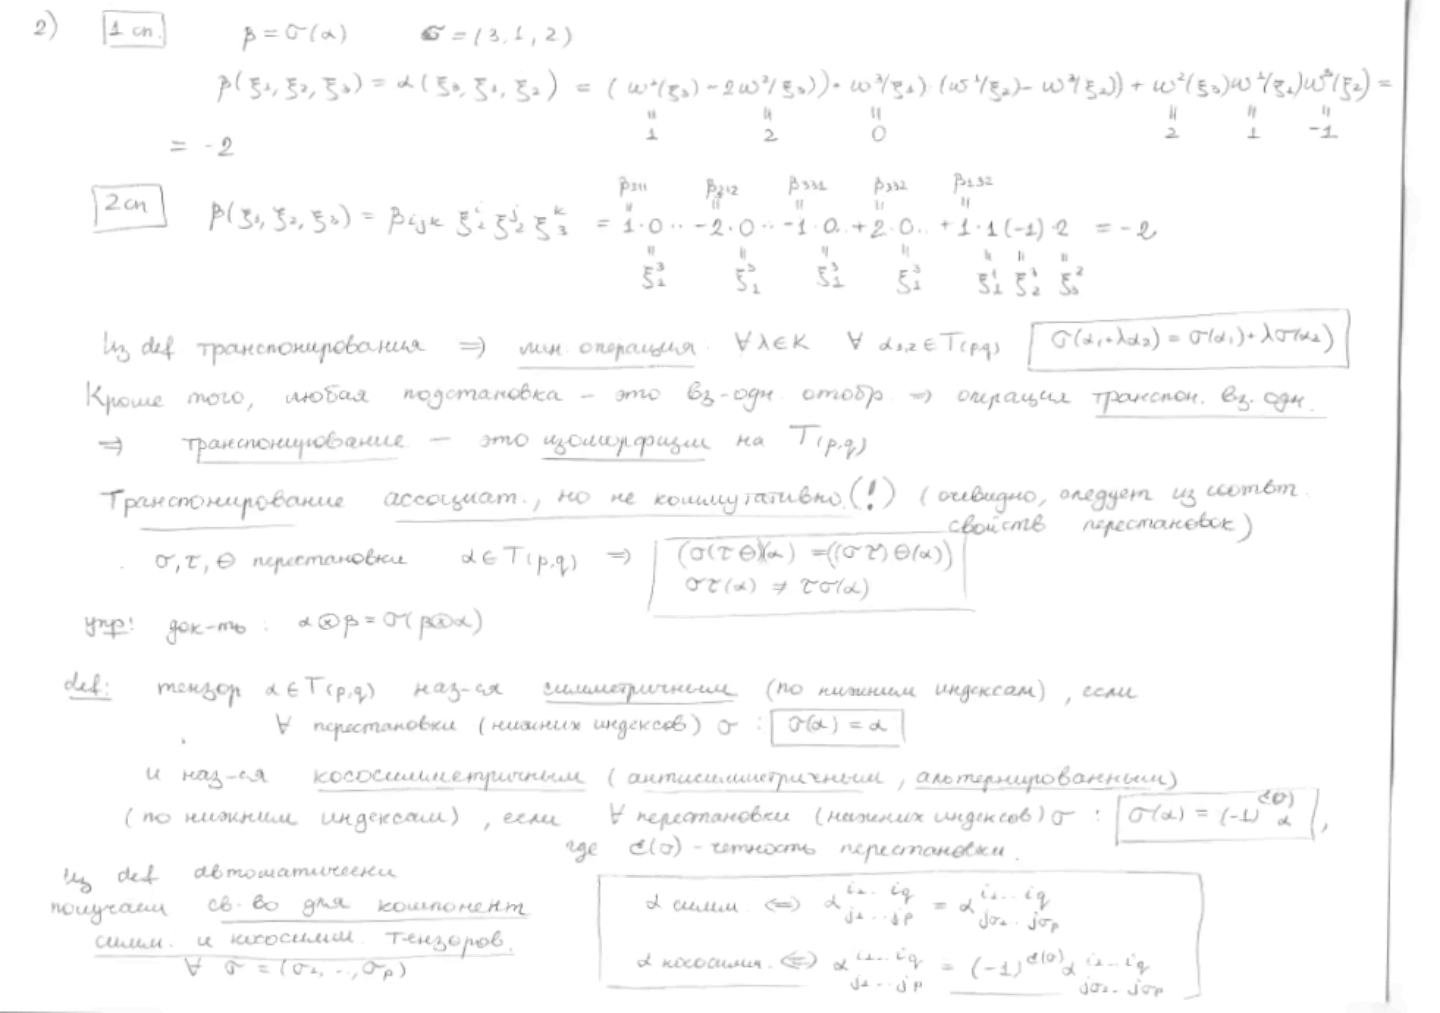
\includegraphics[height=0.49\textheight, width=\textwidth]{new/New_00009}	
		\n
		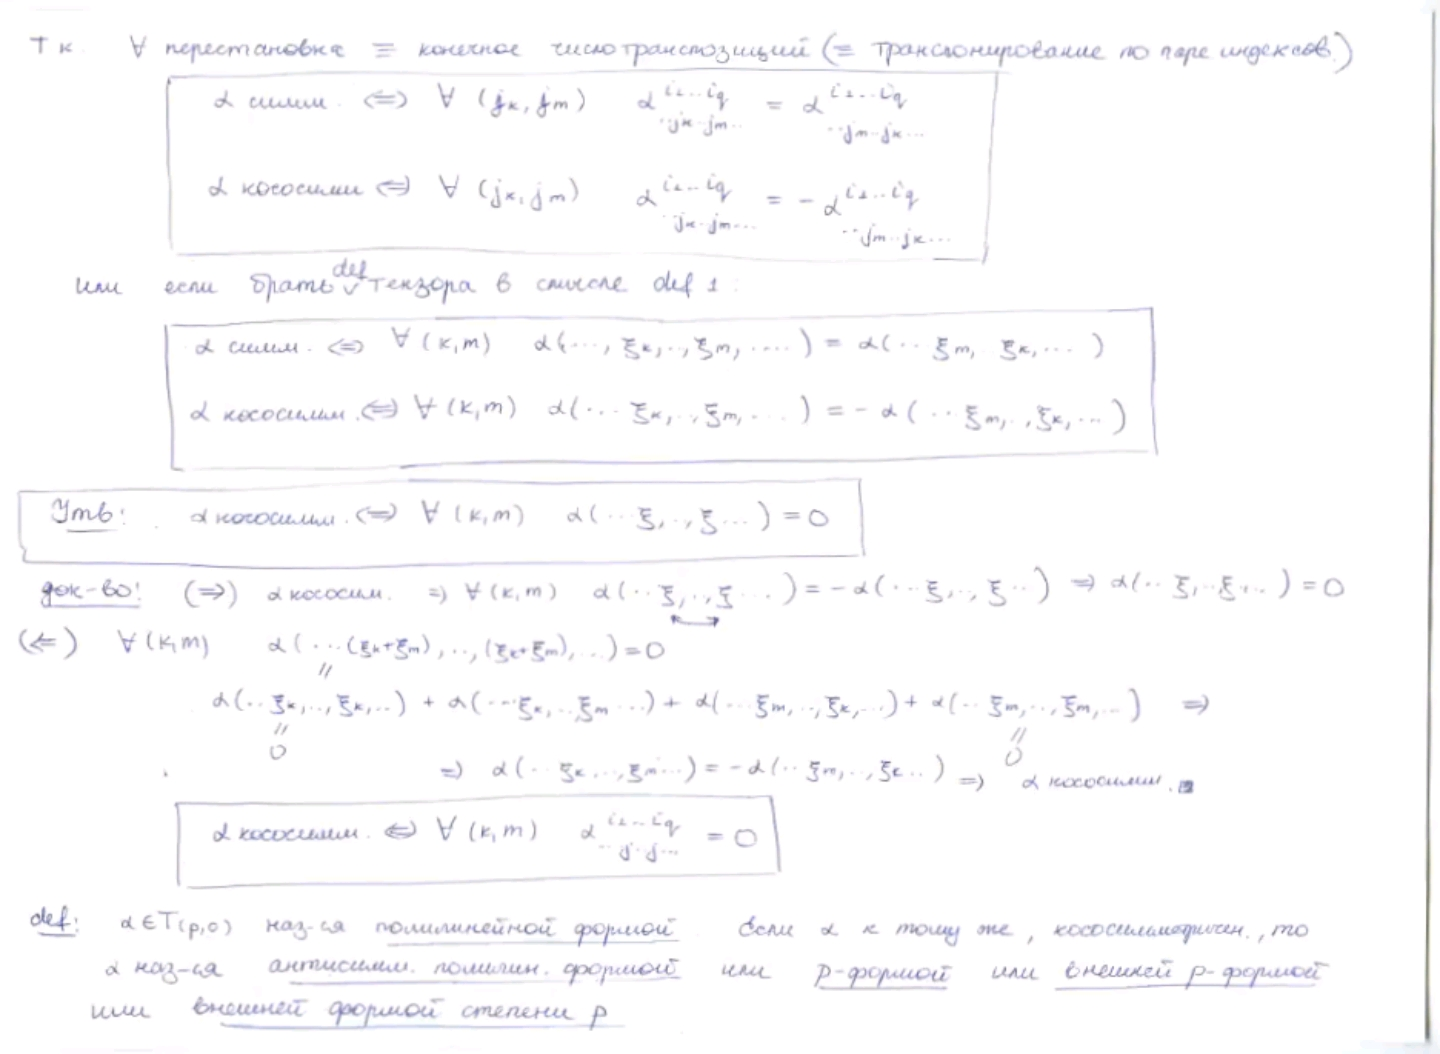
\includegraphics[height=0.49\textheight, width=\textwidth]{new/New_00010}	
		\n
		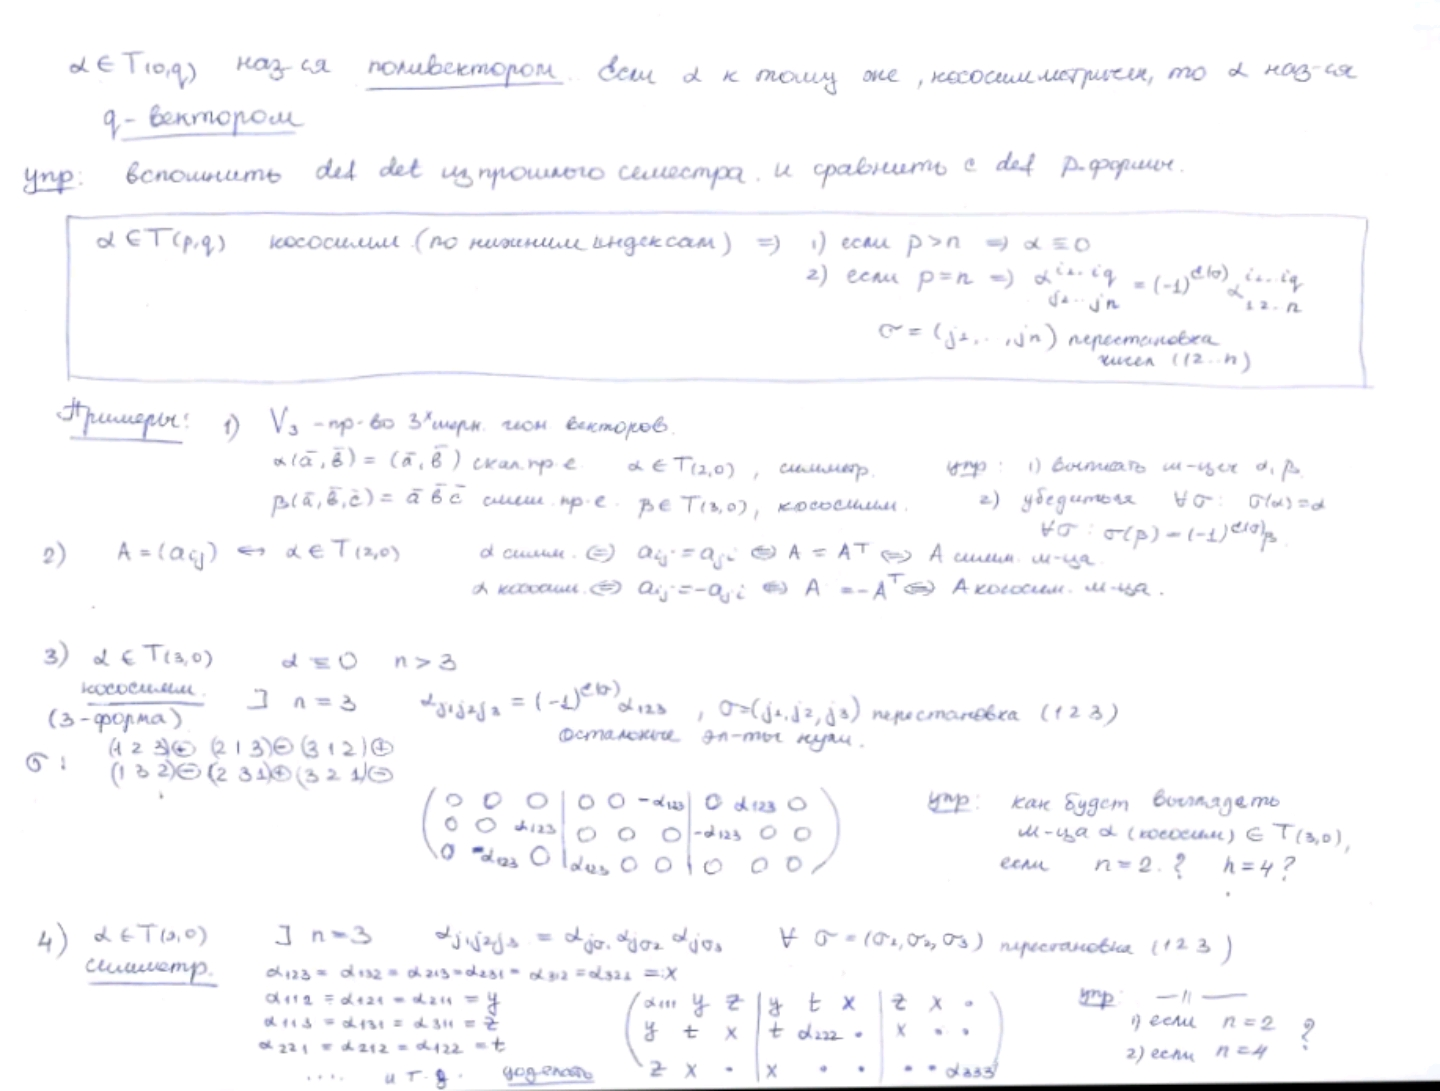
\includegraphics[height=0.49\textheight, width=\textwidth]{new/New_00011}	
		\n			
		
		
	\subsection{Операции альтернирования и симметрирования тензоров}
	 	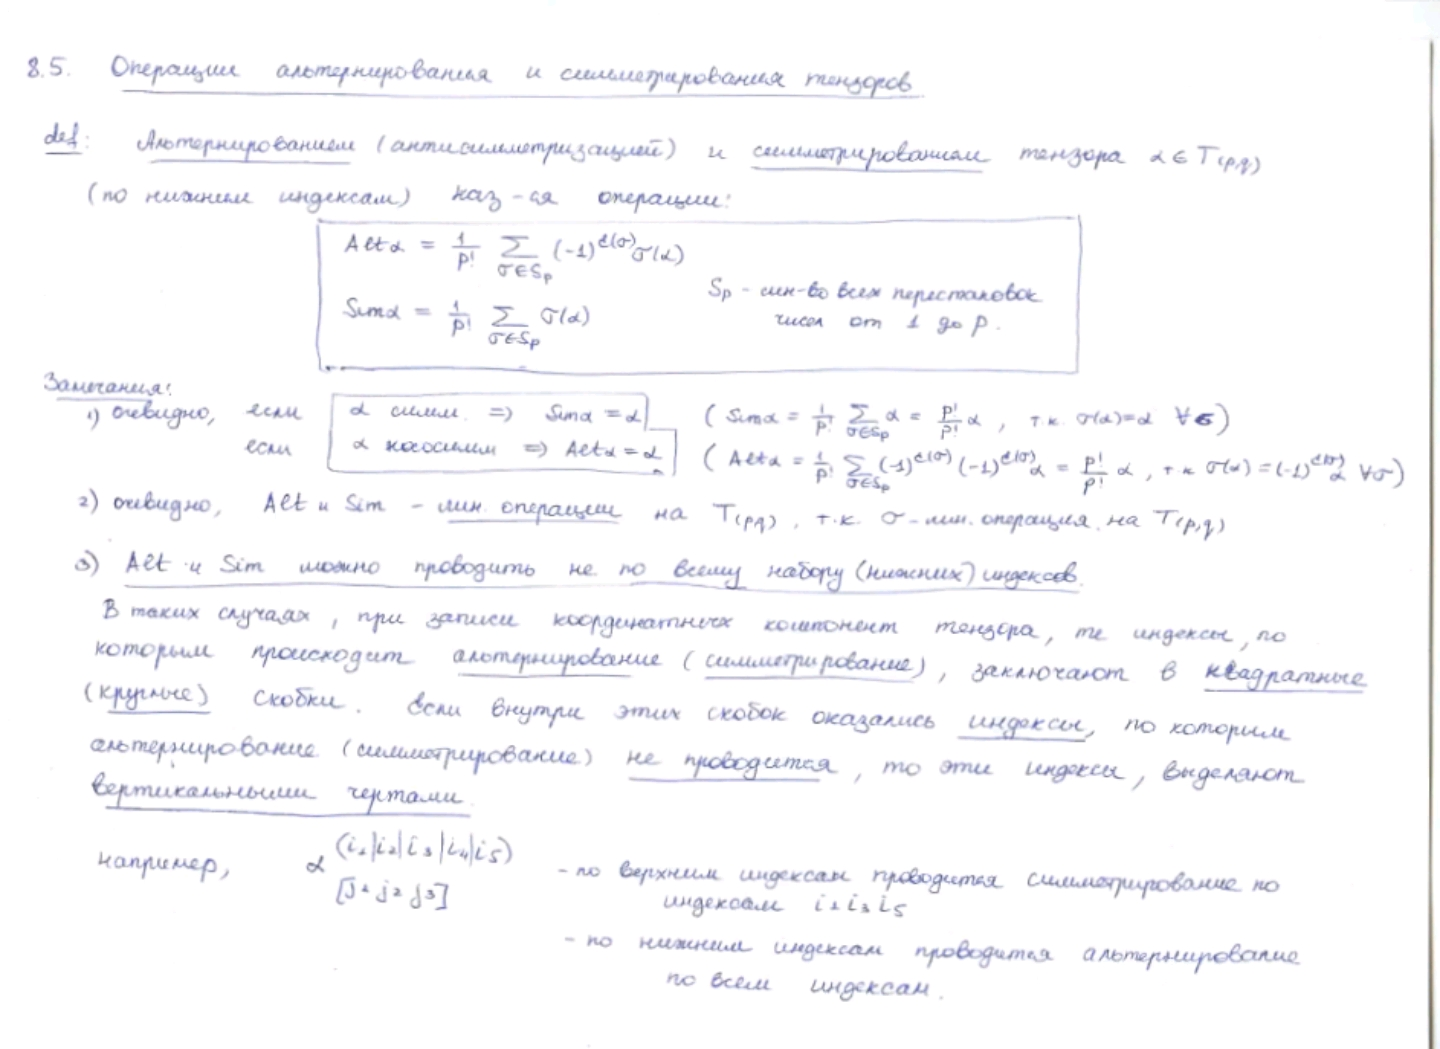
\includegraphics[height=0.49\textheight, width=\textwidth]{new/New_00012}	
		\n
		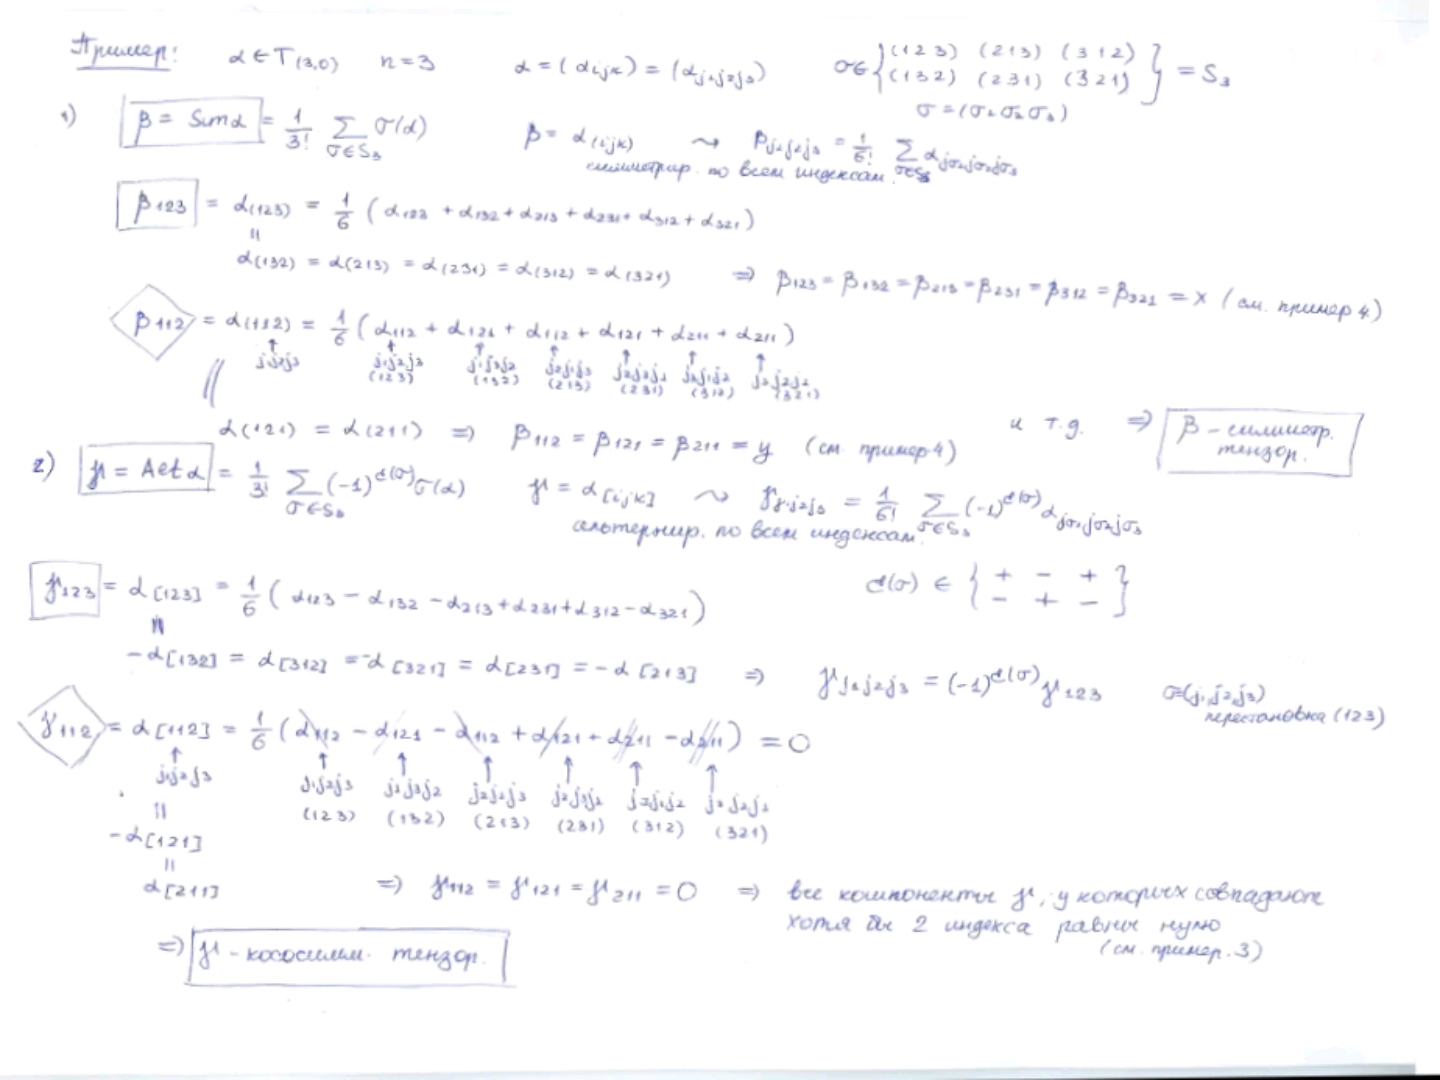
\includegraphics[height=0.49\textheight, width=\textwidth]{new/New_00013}	
		\n
		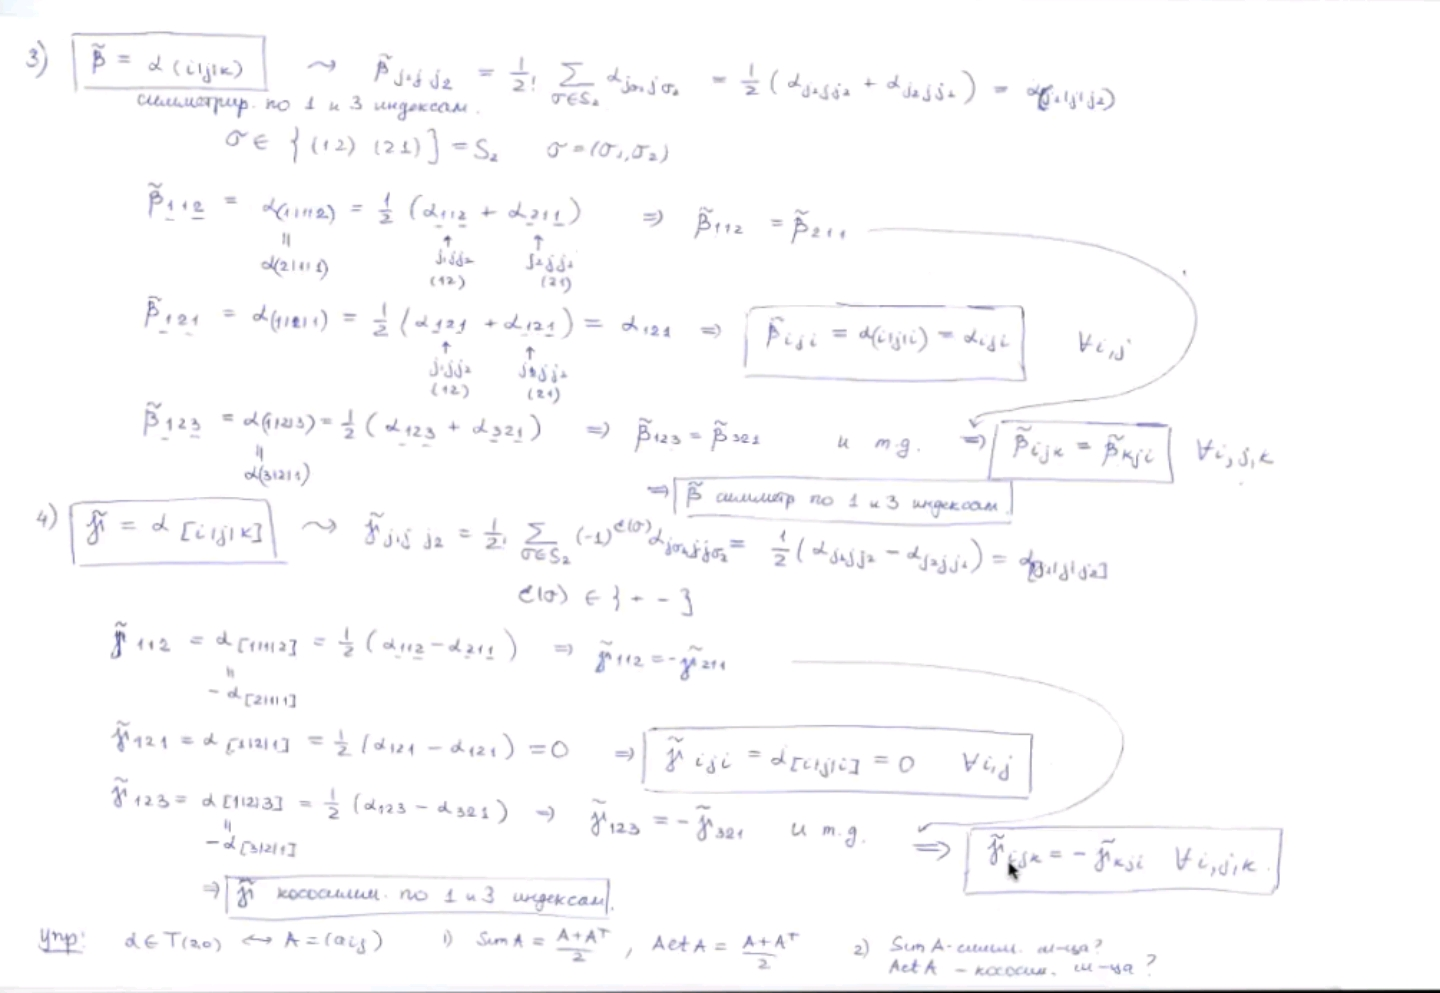
\includegraphics[height=0.49\textheight, width=\textwidth]{new/New_00014}	
\end{document}